\documentclass[11pt,a4paper,final]{article} %draft
\usepackage{pdflscape} % Для использования альбомной ориентации

\usepackage[T1,T2A]{fontenc}
\usepackage[utf8]{inputenc}
\usepackage[english, russian]{babel}

\usepackage[final]{pdfpages}

\usepackage{textcomp,enumitem}

\usepackage{amsmath,amsthm,amssymb}

\usepackage{fancyhdr} % для настройки страницы и колонтитулов
\usepackage{graphicx}
\usepackage{multicol}

\usepackage{indentfirst} % автоматический отступ в начале каждого раздела

\usepackage[unicode, pdftex, colorlinks, urlcolor=blue]{hyperref}

\usepackage[left=2cm,right=2cm,top=2cm,bottom=2cm,bindingo ffset=0cm]{geometry}

\linespread{1.3} % устанавливает междустрочный интервал

\pagestyle{plain} % для отображения номеров внизу

\usepackage{float}

\usepackage{listings} 
\definecolor{darkgreen}{rgb}{0,0.5,0}

\lstset{
	backgroundcolor=\color{lightgray!20},   
	basicstyle=\ttfamily\footnotesize\fontfamily{firamono}\selectfont,
	commentstyle=\color{darkgreen},
	keywordstyle=\color{blue},
	numberstyle=\tiny\color{gray},
	stringstyle=\color{red},
	breakatwhitespace=false,
	breaklines=true,
	captionpos=b,
	keepspaces=true,
	numbers=left,
	numbersep=5pt,
	showspaces=false,
	showstringspaces=false,
	showtabs=false,
	tabsize=4,
	language=python, % Язык программирования
	captionpos=t, % Позиция подписи (b - внизу)
	xleftmargin=0mm, % Отступ слева
	frame=lines, % Тип рамки (single - одинарная, double - двойная, lines - линии)
	framerule=0.25mm, % Толщина рамки
	literate=
	{а}{{\selectfont\char224}}1
	{б}{{\selectfont\char225}}1
	{в}{{\selectfont\char226}}1
	{г}{{\selectfont\char227}}1
	{д}{{\selectfont\char228}}1
	{е}{{\selectfont\char229}}1
	{ж}{{\selectfont\char230}}1
	{з}{{\selectfont\char231}}1
	{и}{{\selectfont\char232}}1
	{й}{{\selectfont\char233}}1
	{к}{{\selectfont\char234}}1
	{л}{{\selectfont\char235}}1
	{м}{{\selectfont\char236}}1
	{н}{{\selectfont\char237}}1
	{о}{{\selectfont\char238}}1
	{п}{{\selectfont\char239}}1
	{р}{{\selectfont\char240}}1
	{с}{{\selectfont\char241}}1
	{т}{{\selectfont\char242}}1
	{у}{{\selectfont\char243}}1
	{ф}{{\selectfont\char244}}1
	{х}{{\selectfont\char245}}1
	{ц}{{\selectfont\char246}}1
	{ч}{{\selectfont\char247}}1
	{ш}{{\selectfont\char248}}1
	{щ}{{\selectfont\char249}}1
	{ъ}{{\selectfont\char250}}1
	{ы}{{\selectfont\char251}}1
	{ь}{{\selectfont\char252}}1
	{э}{{\selectfont\char253}}1
	{ю}{{\selectfont\char254}}1
	{я}{{\selectfont\char255}}1
	{А}{{\selectfont\char192}}1
	{Б}{{\selectfont\char193}}1
	{В}{{\selectfont\char194}}1
	{Г}{{\selectfont\char195}}1
	{Д}{{\selectfont\char196}}1
	{Е}{{\selectfont\char197}}1
	{Ж}{{\selectfont\char198}}1
	{З}{{\selectfont\char199}}1
	{И}{{\selectfont\char200}}1
	{Й}{{\selectfont\char201}}1
	{К}{{\selectfont\char202}}1
	{Л}{{\selectfont\char203}}1
	{М}{{\selectfont\char204}}1
	{Н}{{\selectfont\char205}}1
	{О}{{\selectfont\char206}}1
	{П}{{\selectfont\char207}}1
	{Р}{{\selectfont\char208}}1
	{С}{{\selectfont\char209}}1
	{Т}{{\selectfont\char210}}1
	{У}{{\selectfont\char211}}1
	{Ф}{{\selectfont\char212}}1
	{Х}{{\selectfont\char213}}1
	{Ц}{{\selectfont\char214}}1
	{Ч}{{\selectfont\char215}}1
	{Ш}{{\selectfont\char216}}1
	{Щ}{{\selectfont\char217}}1
	{Ъ}{{\selectfont\char218}}1
	{Ы}{{\selectfont\char219}}1
	{Ь}{{\selectfont\char220}}1
	{Э}{{\selectfont\char221}}1
	{Ю}{{\selectfont\char222}}1
	{Я}{{\selectfont\char223}}1,
	numbers=left, % пронумеровать строки с левой стороны
	breaklines=true % разрешает автоматический перенос строк
}

\hypersetup{
	colorlinks=true, % делает ссылки цветными вместо рамки
	linkcolor=blue, % цвет внутренних ссылок
	urlcolor=blue, % цвет внешних ссылок
	citecolor=blue % цвет ссылок на литературу в тексте
}
\textheight=24cm 
\textwidth=16cm
\oddsidemargin=0pt 
\topmargin=-1.5cm
\parindent=24pt 
\parskip=0pt 
\tolerance=2000 
\flushbottom 

\usepackage{float}

\usepackage{afterpage}

%\usepackage[font=scriptsize]{caption}
\usepackage[labelsep=period]{caption}

\begin{document}
	\thispagestyle{empty}
	
	\begin{center}
		{\Large МИНОБРНАУКИ РОССИИ}\\
		~\\
		{\large ФЕДЕРАЛЬНОЕ ГОСУДАРСТВЕННОЕ БЮДЖЕТНОЕ ОБРАЗОВАТЕЛЬНОЕ УЧРЕЖДЕНИЕ ВЫСШЕГО ПРОФЕССИОНАЛЬНОГО ОБРАЗОВАНИЯ}\\
		~\\
		{\Large \bf <<САНКТ-ПЕТЕРБУРГСКИЙ ПОЛИТЕХНИЧЕСКИЙ УНИВЕРСИТЕТ ПЕТРА ВЕЛИКОГО>>}\\
		~\\
		{\large Институт Компьютерных наук и кибербезопасности }\\
		{\large Высшая школа технологий искусственного интеллекта}\\
		{\large Направление 02.03.01. Математика и компьютерные науки}\\
		~\\
		~\\
		~\\
		~\\
		{ {\LARGE \bf Отчет по курсовой работе}}\\
		\vspace{3mm}
		{\Large {по дисциплине <<Теоретические основы баз данных>>}}\\
		~\\
		{\Large \bf Процесс прохождения кастинга претендентом на роль в фильме }\\
		~\\
		~\\
		~\\
		~\\
		~\\
		{\large Обучающийся: \underline{\hspace{3.5cm}} \hspace{12mm} Шихалев А.О.}\\
		~\\
		{\large Руководитель: \underline{\hspace{3.5cm}} \hspace{12mm} Попов С.Г.}\\
		~\\
		~\\
		~\\
		~\\
	\end{center}
	\begin{flushright}
		
		«\underline{\hspace{1cm}}»\underline{\hspace{3cm}}20\underline{\hspace{0.7cm}}г.
	\end{flushright}
	~\\
	~\\
	
	\begin{center}
		{\large Санкт-Петербург, 2024}
	\end{center}
	
	\newpage
	
\tableofcontents

\newpage	
\section{Аналитика}
\subsection{Описание предметной области}
\par В качестве предметной области был взят процесс прохождения кастинга претендентом на роль в фильме.

\subsubsection{Фильм -- это?}
\par Фильм -- это художественное произведение, имеющее в основе вымышленный сюжет, воплощённый в сценарии и интерпретируемый режиссёром, который создаётся с помощью актёрской игры или средств мультипликации. В процессе создания фильма часто задействованы различные креативные профессионалы, включая режиссёров, сценаристов, актёров, операторов, композиторов и многих других.

\subsubsection{Роль в фильме}
\par Каждый фильм содержит персонажей, которые выполняют определенные роли в сюжете. Роль в фильме может быть главной, второстепенной или эпизодической. 
\par Претенденты на роль (актеры), проходящие кастинг, стремятся получить определенные роли в фильме в соответствии с их навыками, типажами и личными предпочтениями. 

\subsubsection{Что такое кастинг в киноиндустрии?}
\par \textbf{Кастинг} представляет собой отбор среди претендентов человека, в наибольшей мере соответствующего творческому замыслу. В киноиндустрии во время кастинга \textbf{претенденты} представляют свои способности, навыки и таланты перед режиссером и кастинг-директором, чтобы решить, кто лучше всего подходит для определенных ролей. 
\par Для оценки навыков будущего актера введенна балльная система. На каждом этапе кастинга претенденты оцениваются 
профессионалом в киноиндустрии, ответственным за организацию и проведение кастингов для фильмов -- \textbf{кастинг-директором}. Помимо него, в отборе на главные роли участвует и \textbf{режиссер} -- творческий руководитель кинопроекта, ответственный за воплощение задуманной истории на экране. 

\subsubsection{Этапы кастинга}
В процессе кастинга в киноиндустрии обычно выделяются следующие этапы:

\begin{enumerate}
	\item \textbf{Рассмотрение заявки.} Претенденты, которые желают попасть на пробы, отправляют \textbf{заявку} с приложенными к ней фотографиями. Баллы, начисленные за этот этап, могут служить фильтром для отбора наиболее подходящих кандидатов. 
	
	\item \textbf{Одиночные кинопробы.} После успешного рассмотрения заявки, актер может быть приглашен на кинопробу. Претенденту дается заранее роль с текстом, которую необходимо будет исполнить. Он выступает один, демонстрируя свои актерские способности и интерпретацию роли перед кастинг-директором и, в случае главной роли, еще и перед режиссером. 
	По окончании кинопробы претендент получит оценки кастинг-директора и режиссера, которые будут влиять на его позицию в рейтинге и прохождение на следующий этап.
	
	\item \textbf{Парные пробы с партнером по сцене.} Некоторые роли требуют взаимодействия с другими персонажами. В таких случаях актер после успешного прохождения одиночной кинопробы может быть приглашен на парную кинопробу, где он играет сцену с партнером по сцене, что помогает оценить химию между актерами. Аналогично предыдущему этапу, он получит оценку кастинг-директора и режиссера. Помимо вышеперечисленного, на этом этапе происходит подведение итогов - подсчет баллов.  
	
	
\end{enumerate}

\par Баллы, полученные на этих этапах, могут определить, насколько актеры соответствуют требованиям роли и насколько хорошо они сыграли в сцене. Когда подача заявок заканчивается, актер, получивший наибольшее количество баллов, получает роль в фильме. В случае, если наиболее подходящий актер откажется, можно будет легко найти ему замену.  


\newpage

\par \textbf{Роли и их атрибуты:}
\begin{enumerate}

\item \textbf{Актёр} -- это профессиональный исполнитель ролей в кино.

  \begin{itemize}
  	\item Фамилия
  	\item Имя
  	\item Отчество
  	\item Дата рождения
  	\item Номер паспорта
  	\item Образование 
  	\item Опыт работы 
  \end{itemize}

\item \textbf{Режиссер} -- руководящий участник процесса создания фильма, отвечающий за художественную, игровую и сценическую составляющие картины.
  	\begin{itemize}
    	\item Фамилия
    	\item Имя
    	\item Отчество
    	\item Дата рождения
    	\item Номер паспорта
    	\item Фильмы, которые снял
    	\item Фильмы, которые режиссирует
  \end{itemize}

\item \textbf{Кастинг-директор} -- специалист, руководящий процессом подбора и найма актеров для съемок.
  \begin{itemize}
      \item Фамилия
      \item Имя
      \item Отчество
      \item Дата рождения
      \item Номер паспорта
      \item Фильмы, в которые проводил отбор актеров
      \item Фильмы, в которые осуществляет отбор
  \end{itemize}

\end{enumerate}


\par \textbf{Сущности и их атрибуты:}
\begin{enumerate}
		
\item \textbf{Заявка претендента(актера)} -- данные о претенденте на роль в фильме, содержащие информацию о его личных данных, фотографиях, фильмографии, предоставленные в целях участия в кастинге.
  \begin{itemize}
    \item Данные актера
  	\item Фотографии
  	\item Фильмография
  \end{itemize}

\item \textbf{Первый этап(отбор по заявке):} -- этап кастинга, на котором осуществляется первичный отбор актеров на основе их заявок. Здесь оценивается соответствие актеров требованиям роли кандидатом кастинг-директором и режиссером. Также делается решение о переходе на следующий этап кастинга.
\begin{itemize}
	\item Данные заявки
	\item Оценка кастинг-директора
	\item Оценка режиссера
	\item Прошел ли на второй этап? 
	
\end{itemize}

\item \textbf{Второй этап(прослушивание):} -- вторая стадия кастинга, где претенденты, прошедшие первый этап, проходят прослушивание перед кастинг-директором и режиссером. Оценка проводится на основе игровых навыков и соответствия роли.
\begin{itemize}
	\item Данные заявки
	\item Оценка кастинг-директора
	\item Оценка режиссера
	\item Прошел ли на финальный этап?
\end{itemize}

\item \textbf{Финальный этап (парные пробы):} -- последний этап кастинга, где финальные кандидаты проходят парные пробы, играя с другими актерами, которые уже выбраны для ролей. Здесь проводится окончательная оценка и принимается решение о выборе актера на роль.
\begin{itemize} 
	\item Данные заявки
	\item Оценка кастинг-директора
	\item Оценка режиссера
	\item Общее количество баллов 
	\item Получил роль? 
\end{itemize}


\item \textbf{Фильм:} -- отдельное кинематографическое произведение, содержащее название, список жанров и перечень ролей, которые требуется заполнить актерами.
\begin{itemize}
	\item Название фильма 
	\item Жанры фильма 
	\item Список названия ролей 
\end{itemize}

\item \textbf{Жанры:} -- категории, в которые можно классифицировать фильмы в зависимости от их характеристик и тематики.
\begin{itemize}
	\item Название  

\end{itemize}

\item \textbf{Роль:} -- характеристики конкретной роли в фильме, включая данные об актере, который её займет, данные о заявке, фильме, название и описание роли, а также её тип.
\begin{itemize}
	\item Данные актёра
	\item Данные заявки 
	\item Фильм 
	\item Название роли
	\item Тип роли(главная, второстепеннная, эпизодическая)
	\item Описание роли 
\end{itemize}

\item \textbf{Тип роли:} --  классификация ролей в фильме по их значимости и объему участия в сюжете. 
\begin{itemize}
	\item Название  
\end{itemize}

\end{enumerate}
 

\subsection {ER-диаграмма}
\par ER-диаграмма кастинга актеров представлена на рис. 1.
\par \textbf{Чтение ER-диаграммы.}

\par Актёр может подать одну или несколько заявок на роль.
\par Роли содержатся в фильмах.
\par У каждой роли есть свой тип (главная, второстепенная, эпизодическая).
\par Фильмы включают в себя один или несколько жанров.
\par Актёр проходит 3 этапа:
\begin{itemize}[itemindent=2em]
	\item Первый этап (фотоотбор)
	\item Прослушивание
	\item Парные пробы
\end{itemize}
\par К каждой заявке привязаны этапы в зависимости от их прохождения актером.
\par Все этапы проводятся режиссером и кастинг-директором.

\newpage
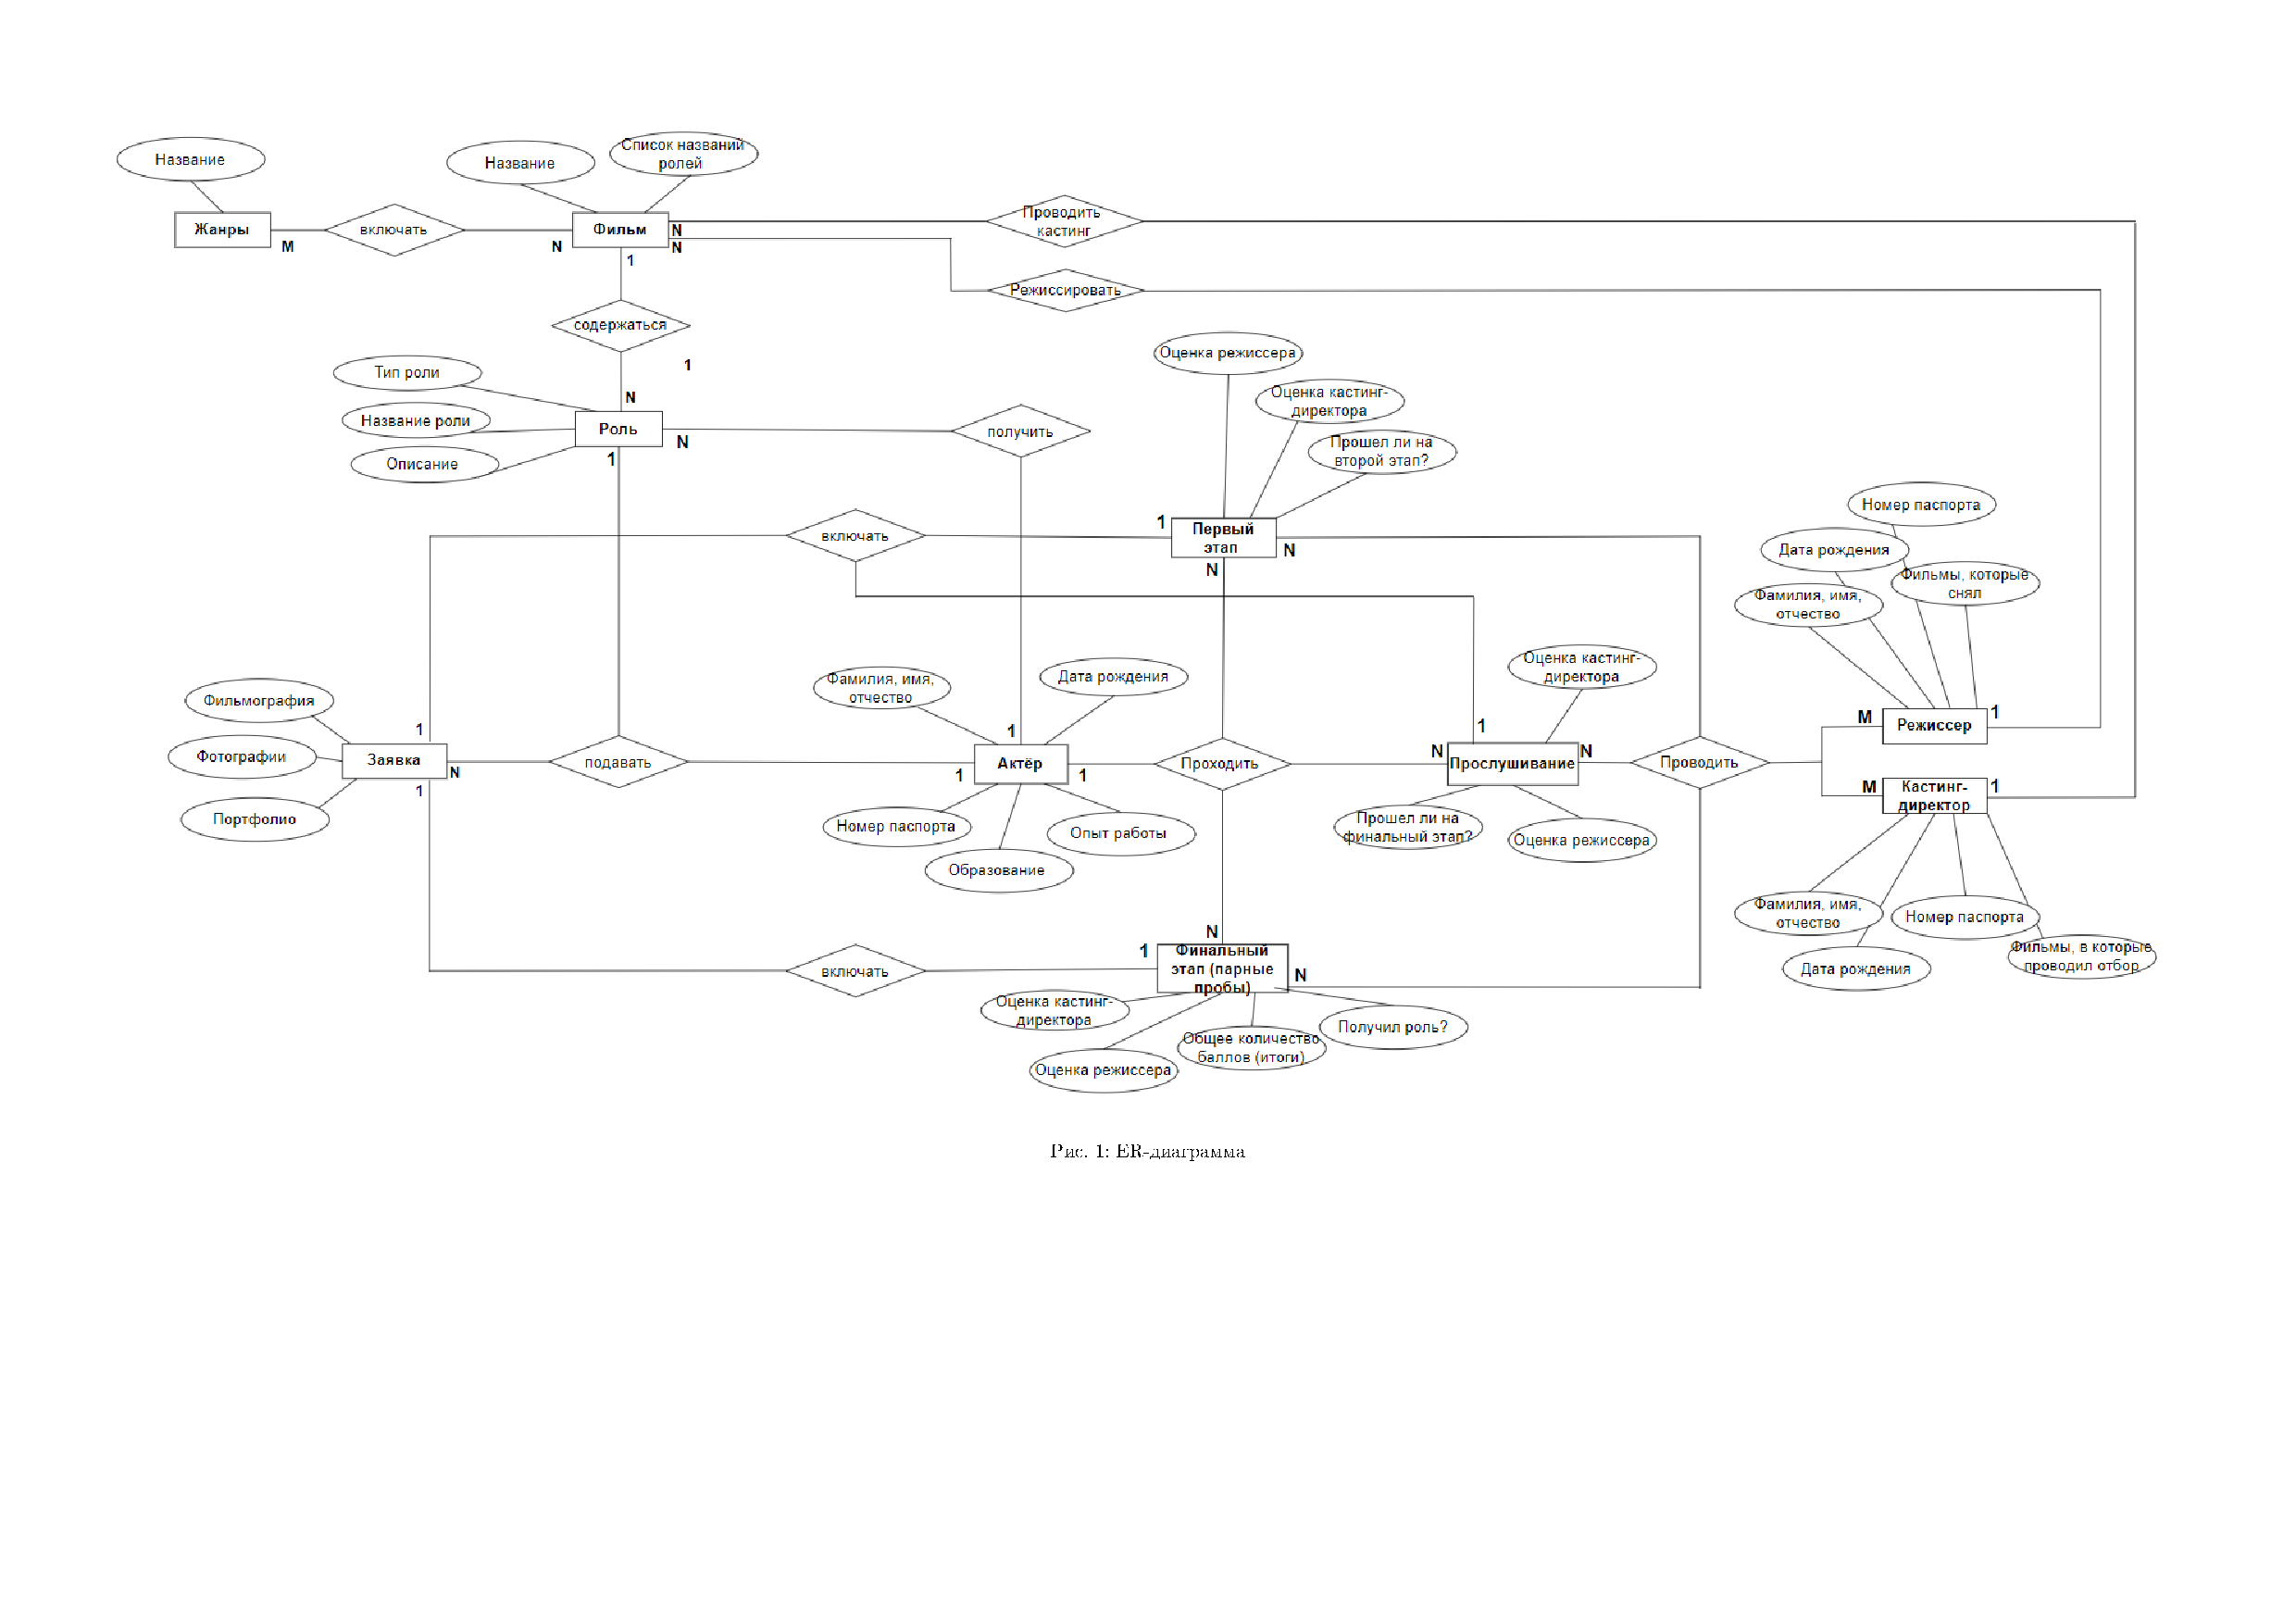
\includepdf[pages=-,fitpaper]{er.pdf}
\setcounter{figure}{1}

\newpage 
\section{Проектирование}

\subsection{Цели функционирования базы данных}
\begin{enumerate}
	\item Учет и выбор наиболее подходящих претендентов для каждой роли в фильме. 
	\item Найти замену актеру, выбывшего из кинопроекта. 
	\item Посмотреть историю кастингов актера. 
	\item История участия актеров в фильме.
\end{enumerate}


\subsection{Cхема базы данных}
\par Схема базы данных на русском языке представлена на рис.3.
\par Схема базы данных на английском языке представлена на рис.4.

\subsection{Диаграмма объектов}

\begin{figure}[H]
	\centering
	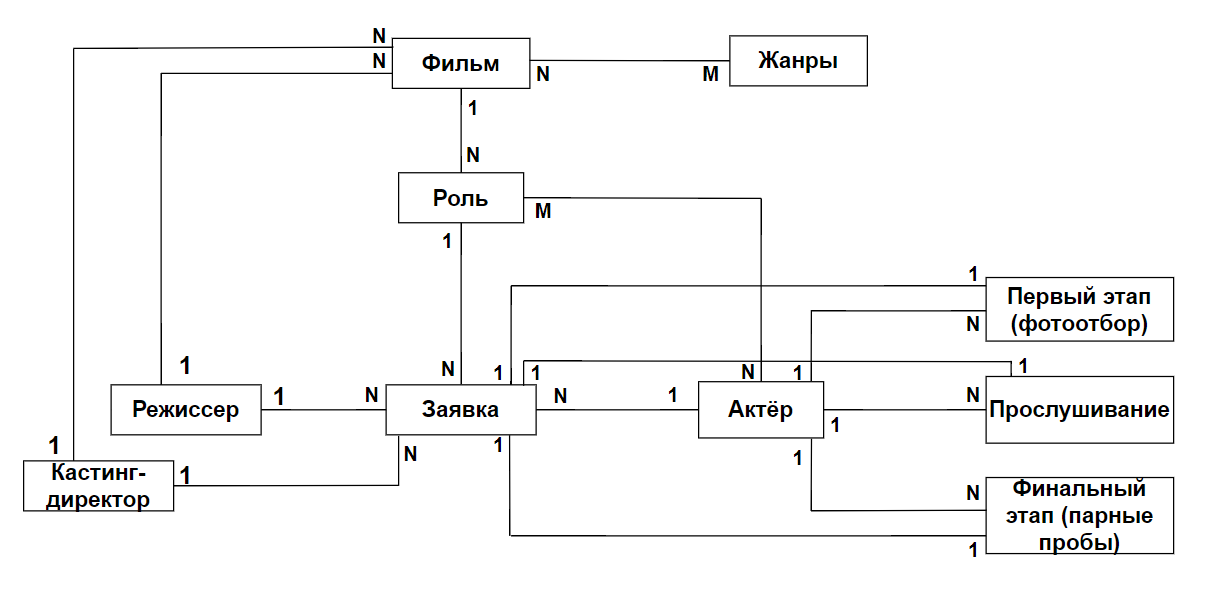
\includegraphics[width=1.0\linewidth]{diagram.png}
	\caption{Диграмма объектов}
	\label{fig:diagram}
\end{figure}

\newpage
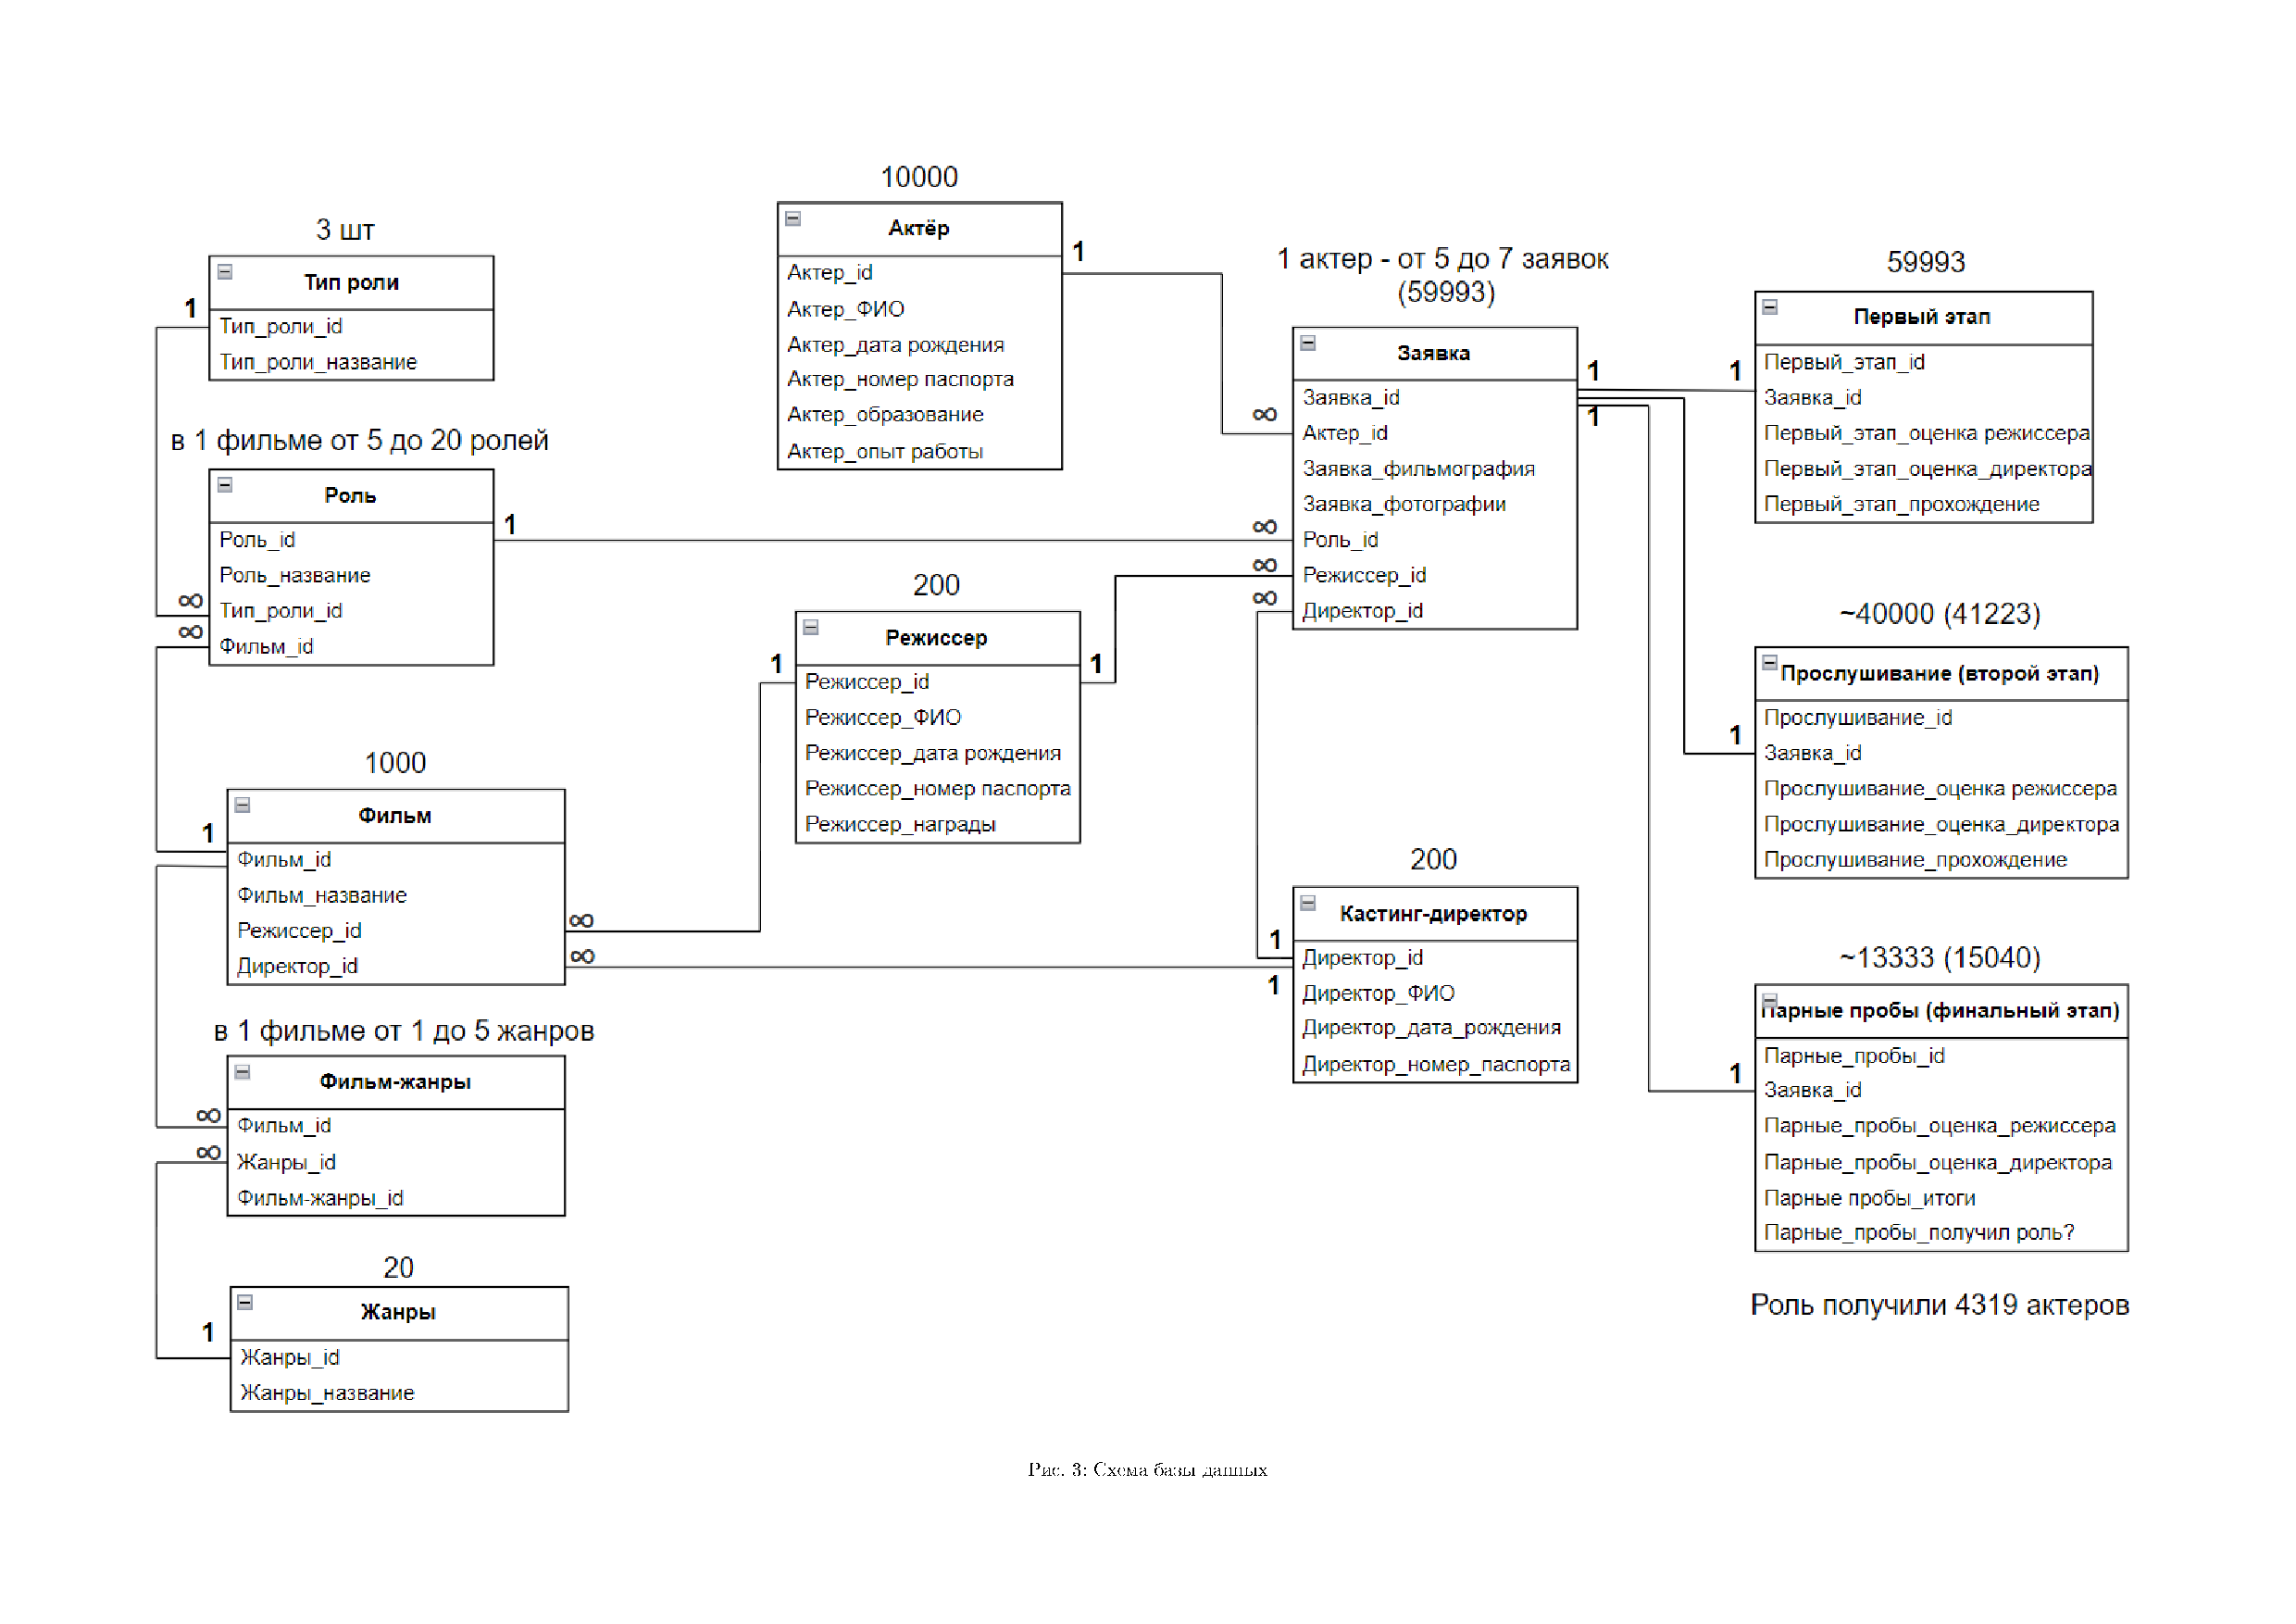
\includepdf[pages=-,fitpaper]{а3.pdf} % Вставка документа формата A3  
\setcounter{figure}{4}

\newpage
\subsection{Таблицы связи базы данных}
\vspace{-\baselineskip} 
\begin{table}[H]
	\centering
	\begin{tabular}{|c|p{2.8cm}|c|c|p{2cm}|c|}
		\hline
		& Название ENG & Название RUS & Тип атрибута & NULL\textbackslash \newline NOT NULL & REFERENCES \\
		\hline
		PRI & id\_actor & id\_актер & int unsigned & NOT NULL &  \\
		\hline
		& surname & фамилия & varchar(30) & NULL & \\
		\hline
		& name & имя & varchar(20) & NULL &  \\
		\hline
		& patronymic & отчество & varchar(20) & NULL &  \\
		\hline
		& date\_of\_birth & дата\_рождения & date & NULL &  \\
		\hline
		& passport\_number & номер\_паспорта & varchar(15) & NULL &  \\
		\hline
		& education & образование & varchar(100) & NULL &  \\
		\hline
		& work\_experience & опыт\_работы & varchar(100) & NULL &  \\
		\hline
	\end{tabular}
	\caption{Актёр}
	\label{tab:actor}
\end{table}
\par Сегодня самой длинной русской фамилией считается Христорождественская, состоящая из 20 букв. Если мы предположим возможность сдвоенности длинных фамилий, то длина может превысить 20 символов, поэтому возьмём с запасом - 30 символов. Самым длинным именем считается Абдурахмангаджи (15 символов). С запасом - 20 символов. Отчество не может сильно превышать самое длинное имя, поэтому оставим тоже 20 символов. 

\par Тип date предназначен для хранения даты в формате YYYY-MM-DD, поэтому идеально подходит для даты рождения. Для passport\_number выбран тип varchar(15), поскольку в паспортах могут встречаться как цифры, так и буквы. Для education и work\_experience был выбран тип varchar(100) потому, что он обеспечивает достаточное пространство для хранения длинных текстовых данных, но не такими огромными, чтобы требовать большего объема памяти. 

\begin{table}[H]
	\centering
	\begin{tabular}{|c|p{2.8cm}|p{2.5cm}|c|p{2cm}|p{3.5cm}|}
		\hline
		& Название ENG & Название RUS & Тип атрибута & NULL\textbackslash \newline NOT NULL & REFERENCES \\
		\hline
		PRI & id\_application & id\_заявка & int unsigned & NOT NULL &  \\
		\hline
		& filmography & фильмография & varchar(100) & NULL & \\
		\hline
		& photos & фотографии & varchar(200) & NULL &  \\
		\hline
		FK & id\_actor & id\_актер & int unsigned & NOT NULL & actor(id\_actor) \\
		\hline
		FK & id\_role & id\_роль & int unsigned & NOT NULL & role(id\_role) \\
		\hline
		FK & id\_сasting\_\newline director & id\_кастинг\_ \newline директор & int unsigned & NOT NULL & casting\_director (id\_casting\_director) \\
		\hline
		FK & id\_director & id\_режиссер & int unsigned & NOT NULL & director(id\_director) \\
		\hline
	\end{tabular}
	\caption{Заявка}
    \label{tab:application}
\end{table}

\par Для фильмографии выбран тип varchar(100), поскольку фильмография актера может быть достаточно большой.

\begin{table}[H]
	\centering
	\begin{tabular}{|c|p{2.8cm}|p{2.8cm}|c|p{2cm}|p{2.5cm}|}
		\hline
		& Название ENG & Название RUS & Тип атрибута & NULL\textbackslash \newline NOT NULL & REFERENCES \\
		\hline
		PRI & id\_director & id\_режиссер & int unsigned & NOT NULL &  \\
		\hline
		& surname & фамилия & varchar(30) & NULL & \\
		\hline
		& name & имя & varchar(20) & NULL &  \\
		\hline
		& patronymic & отчество & varchar(20) & NULL &  \\
		\hline
		& date\_of\_birth & дата\_рождения & date & NULL &  \\
		\hline
		& passport\_number & номер\_паспорта & varchar(15) & NULL &  \\
		\hline
		& awards & награды & varchar(100) & NULL & \\
		\hline
	\end{tabular}
	\caption{Режиссер}
	\label{tab:director}
\end{table}

\vspace{-\baselineskip}

\begin{table}[H]
	\centering
	\begin{tabular}{|c|p{2.8cm}|p{2.8cm}|c|p{2cm}|p{2.5cm}|}
		\hline
		& Название ENG & Название RUS & Тип атрибута & NULL\textbackslash \newline NOT NULL & REFERENCES \\
		\hline
		PRI & id\_casting\_ \newline director & id\_кастинг\_ \newline директор & int unsigned & NOT NULL &  \\
		\hline
		& surname & фамилия & varchar(30) & NULL & \\
		\hline
		& name & имя & varchar(20) & NULL &  \\
		\hline
		& patronymic & отчество & varchar(20) & NULL &  \\
		\hline
		& date\_of\_birth & дата\_рождения & date & NULL &  \\
		\hline
		& passport\_number & номер\_паспорта & varchar(15) & NULL &  \\
		\hline
	\end{tabular}
	\caption{Кастинг-директор}
	\label{tab:cdirector}
\end{table}

\vspace{-\baselineskip}
	
\begin{table}[H]
	\centering
	\begin{tabular}{|c|p{2.8cm}|p{2.5cm}|c|p{2cm}|p{3.5cm}|}
		\hline
		& Название ENG & Название RUS & Тип атрибута & NULL\textbackslash \newline NOT NULL & REFERENCES \\
		\hline
		PRI & id\_role & id\_роль  & int unsigned & NOT NULL &  \\
		\hline
		& name & название & varchar(30) & NULL & \\
		\hline
		FK & id\_role\_type & id\_тип\_роли & int unsigned & NOT NULL & role\_type \newline (id\_role\_type) \\
		\hline
		FK & id\_film & id\_фильм & int unsigned & NOT NULL & film(id\_film) \\
		\hline
	\end{tabular}
	\caption{Роль}
	\label{tab:role}
\end{table}
	

\begin{table}[H]
	\centering
	\begin{tabular}{|c|p{2.8cm}|p{2.5cm}|c|p{2cm}|p{3.5cm}|}
		\hline
		& Название ENG & Название RUS & Тип атрибута & NULL\textbackslash \newline NOT NULL & REFERENCES \\
		\hline
		PRI & id\_role\_type & id\_тип\_роли & int unsigned & NOT NULL &  \\
		\hline
		& name & название & varchar(15) & NULL & \\
		\hline
	\end{tabular}
	\caption{Тип роли}
	\label{tab:roletype}
\end{table}
	
\begin{table}[H]
	\centering
	\begin{tabular}{|c|p{2.8cm}|p{2.5cm}|c|p{2cm}|p{3.5cm}|}
		\hline
		& Название ENG & Название RUS & Тип атрибута & NULL\textbackslash \newline NOT NULL & REFERENCES \\
		\hline
		PRI & id\_film & id\_фильм  & int unsigned & NOT NULL &  \\
		\hline
		& name & название & varchar(30) & NULL & \\
		\hline
		FK & id\_сasting\_\newline director & id\_кастинг\_ \newline директор  & int unsigned & NOT NULL & casting\_director (id\_casting\_director) \\
        \hline
        FK & id\_director & id\_режиссер & int unsigned & NOT NULL & director(id\_director) \\
        \hline
	\end{tabular}
	\caption{Фильм}
	\label{tab:film}
\end{table}		
	
	
\begin{table}[H]
	\centering
	\begin{tabular}{|c|p{2.8cm}|p{2.5cm}|c|p{2cm}|p{3.5cm}|}
		\hline
		& Название ENG & Название RUS & Тип атрибута & NULL\textbackslash \newline NOT NULL & REFERENCES \\
		\hline
		PRI & id\_film\_ \newline genres & id\_фильм\_ жанры & int unsigned & NOT NULL &  \\
		\hline
		FK & id\_film & id\_фильм & int unsigned & NOT NULL & film(id\_film) \\
		\hline
	    FK & id\_genres & id\_жанры & int unsigned & NOT NULL & genres(id\_genres) \\
		\hline
	\end{tabular}
	\caption{Фильм-жанры}
	\label{tab:filmgenres}
\end{table}	


\begin{table}[H]
	\centering
	\begin{tabular}{|c|p{2.8cm}|p{2.5cm}|c|p{2cm}|p{3.5cm}|}
		\hline
		& Название ENG & Название RUS & Тип атрибута & NULL\textbackslash \newline NOT NULL & REFERENCES \\
		\hline
		PRI & id\_genres & id\_жанры  & int unsigned & NOT NULL &  \\
		\hline
		& name & название & varchar(20) & NULL & \\
		\hline
	\end{tabular}
	\caption{Жанры}
	\label{tab:genres}
\end{table}		
	

\begin{table}[H]
	\centering
	\begin{tabular}{|c|p{3cm}|p{3cm}|c|p{2cm}|p{2.6cm}|}
		\hline
		& Название ENG & Название RUS & Тип атрибута & NULL\textbackslash \newline NOT NULL & REFERENCES \\
		\hline
		PRI & id\_first\_stage & id\_первый\_этап & int unsigned & NOT NULL &  \\
		\hline
		& directors\_ \newline assessment & оценка\_ \newline режиссера & tinyint unsigned & NULL & \\
		\hline
		& casting\_directors\_ \newline assessment & оценка\_кастинг\_ \newline директора & tinyint unsigned & NULL & \\
		\hline
		FK & id\_application & id\_заявка & int unsigned & NOT NULL & application (id\_application) \\
		\hline
	\end{tabular}
	\caption{Первый этап}
	\label{tab:firstStage}
\end{table}	



\begin{table}[H]
	\centering
	\begin{tabular}{|c|p{3cm}|p{3cm}|c|p{2cm}|p{2.6cm}|}
		\hline
		& Название ENG & Название RUS & Тип атрибута & NULL\textbackslash \newline NOT NULL & REFERENCES \\
		\hline
		PRI & id\_audition & id\_прослушивание & int unsigned & NOT NULL &  \\
		\hline
		& directors\_ \newline assessment & оценка\_ \newline режиссера & tinyint unsigned & NULL & \\
		\hline
		& casting\_directors\_ \newline assessment & оценка\_кастинг\_ \newline директора & tinyint unsigned & NULL & \\
		\hline
		FK & id\_application & id\_заявка & int unsigned & NOT NULL & application (id\_application) \\
		\hline
	\end{tabular}
	\caption{Прослушивание}
	\label{tab:audition}
\end{table}	


\begin{table}[H]
	\centering
	\begin{tabular}{|c|p{3cm}|p{3cm}|c|p{2cm}|p{2.6cm}|}
		\hline
		& Название ENG & Название RUS & Тип атрибута & NULL\textbackslash \newline NOT NULL & REFERENCES \\
		\hline
		PRI & id\_doubles\_ \newline audition & id\_парные\_ \newline пробы & int unsigned & NOT NULL &  \\
		\hline
		& directors\_ \newline assessment & оценка\_ \newline режиссера & tinyint unsigned & NULL & \\
		\hline
		& casting\_directors\_ \newline assessment & оценка\_кастинг\_ \newline директора & tinyint unsigned & NULL & \\
		\hline
		FK & id\_application & id\_заявка & int unsigned & NOT NULL & application (id\_application) \\ 
		\hline
	\end{tabular}
	\caption{Парные пробы}
	\label{tab:doubaudition}
\end{table}	

\subsection{Создание БД}
\par По таблицам метаданных был сформирован код с использованием языка определения данных для создания базы данных casting и создания каждой из таблиц в ней. Код представлен в \hyperref[sec:appendixA]{приложении A. Текст создания БД}. Далее последовало написание программы на языке Python с использованием библиотеки pymysql для заполнения созданных таблиц в соответствии с полученным количеством записей по каждой из таблиц. Код заполнения базы данных представлен в \hyperref[sec:appendixB]{приложении Б. Текст программы для заполнения таблиц в БД.}

\newpage
\section{Запросы}	

\subsection{Запрос № 1}

\par \textbf{Текст запроса на русском}: Для актера А найти все заявки, которые он подавал на фильм жанра Б. 
\par Текст SQL запроса представлен в листинге 1.

\begin{lstlisting}[caption=SQL запрос № 1, language=SQL]
		
SELECT 
a.id_actor,
CONCAT(a.surname, ' ', a.name) AS actor_name,
GROUP_CONCAT(ap.id_application) AS id_application,
GROUP_CONCAT(DISTINCT r.name) AS roles_in_applications,
GROUP_CONCAT(DISTINCT f.name) AS films_for_roles,
GROUP_CONCAT(DISTINCT g.name) AS genres
FROM 
actor a
LEFT JOIN 
application ap ON a.id_actor = ap.id_actor
LEFT JOIN 
role r ON ap.id_role = r.id_role
LEFT JOIN 
film f ON r.id_film = f.id_film
LEFT JOIN 
film_genres fg ON f.id_film = fg.id_film
LEFT JOIN 
genres g ON fg.id_genres = g.id_genres
WHERE 
a.name = 'Алексей' AND a.surname = 'Шихалев' AND g.name = 'Байопик'
GROUP BY 
ap.id_application, actor_name;
	
\end{lstlisting}
 

В качестве результата выполнения запроса была получена таблица на 2 строки. Запрос выполнился за 0.0104 секунд. Заголовок таблицы и несколько кортежей представлены на \autoref{fig:1}.

	\begin{figure}[H]
	\centering
	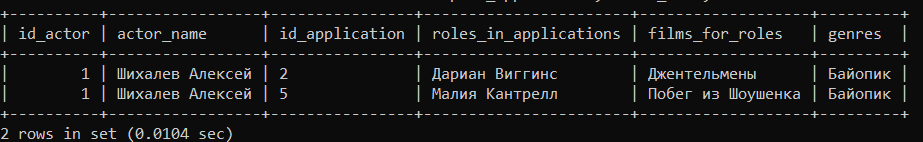
\includegraphics[width=1.0\linewidth]{1.png}
	\caption{Результат выполнения запроса № 1}
	\label{fig:1}
\end{figure}

\begin{figure}[H]
	\centering
	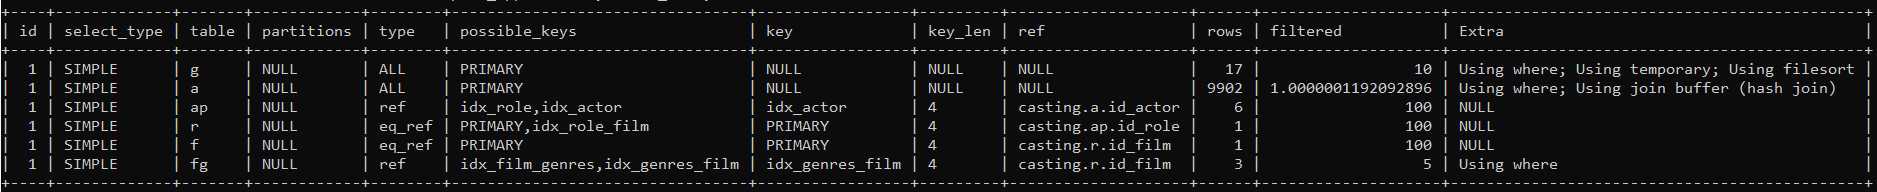
\includegraphics[width=1.0\linewidth]{e1.png}
	\caption{Результат применения команды explain к данному запросу}
	\label{fig:e1}
\end{figure}

\begin{figure}[H]
	\centering
	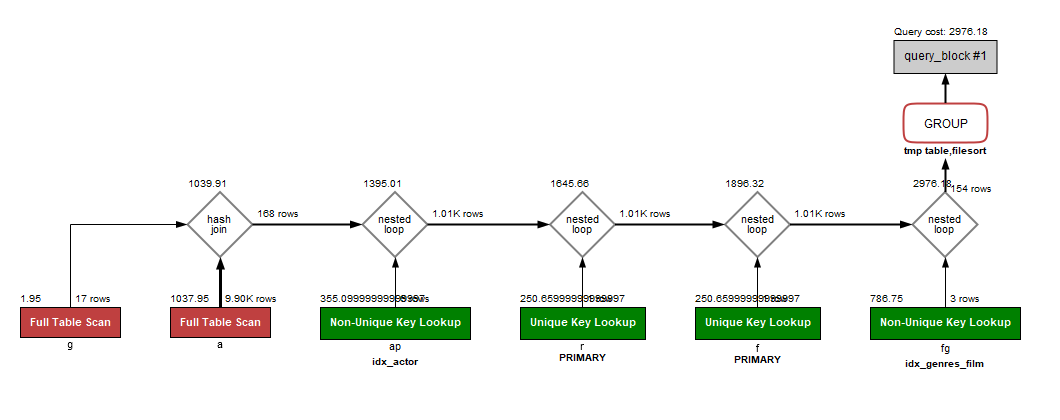
\includegraphics[width=1.0\linewidth]{ex1.png}
	\caption{Графический план выполнения запроса № 1.}
	\label{fig:ex1}
\end{figure}

\subsection{Запрос № 2}

\par \textbf{Текст запроса на русском}: Для режиссера А подсчитать число заявок, поданных на роль типа Б. 
\par Текст SQL запроса представлен в листинге 2.

\begin{lstlisting}[caption=SQL запрос № 2, language=SQL]
SELECT
CONCAT(d.surname, ' ', d.name) AS director_name,
GROUP_CONCAT(DISTINCT rt.name) AS role_type,
COUNT(ap.id_application) AS num_applications 
FROM director d
JOIN application ap ON d.id_director = ap.id_director
JOIN role r ON ap.id_role = r.id_role
JOIN role_type rt ON r.id_role_type = rt.id_role_type 
WHERE d.id_director = 2 AND rt.name = 'Главная';
\end{lstlisting}


В качестве результата выполнения запроса была получена строка, в которой представлено имя и фамилия режиссера, тип роли и количество заявок. Запрос выполнился за 0.0023 секунд. Заголовок таблицы и несколько кортежей представлены на \autoref{fig:2}.

\begin{figure}[H]
	\centering
	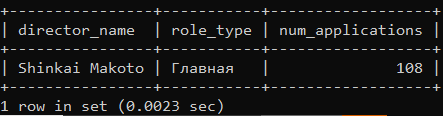
\includegraphics[width=0.7\linewidth]{2.png}
	\caption{Результат выполнения запроса № 2}
	\label{fig:2}
\end{figure}


\begin{figure}[H]
	\centering
	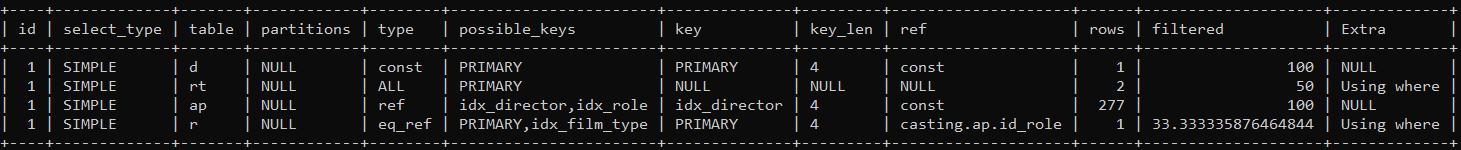
\includegraphics[width=1.0\linewidth]{e2.png}
	\caption{Результат применения команды explain к данному запросу}
	\label{fig:e2}
\end{figure}

\begin{figure}[H]
	\centering
	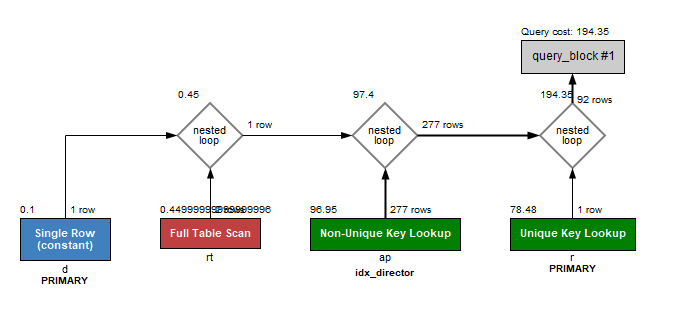
\includegraphics[width=1.0\linewidth]{ex2.png}
	\caption{Графический план выполнения запроса № 2.}
	\label{fig:ex2}
\end{figure}


\subsection{Запрос № 3.1}

\par \textbf{Текст запроса на русском}: Для каждого жанра подсчитать число заявок, поданных на фильмы. 
\par Текст SQL запроса представлен в листинге 3.

\begin{lstlisting}[caption=SQL запрос № 3.1, language=SQL]
	SELECT g.name AS genre_name, COUNT(ap.id_application) AS num_applications
	FROM application ap
	LEFT JOIN role r ON ap.id_role = r.id_role
	LEFT JOIN film f ON r.id_film = f.id_film
	LEFT JOIN film_genres fg ON f.id_film = fg.id_film
	LEFT JOIN genres g ON fg.id_genres = g.id_genres
	GROUP BY g.id_genres, g.name;
\end{lstlisting}

\par В качестве результата выполнения запроса была получена таблица на 20 строк. Запрос выполнился за 0.7674 секунд. Таблица с результатами представлена на \autoref{fig:31}.

\begin{figure}[H]
	\centering
	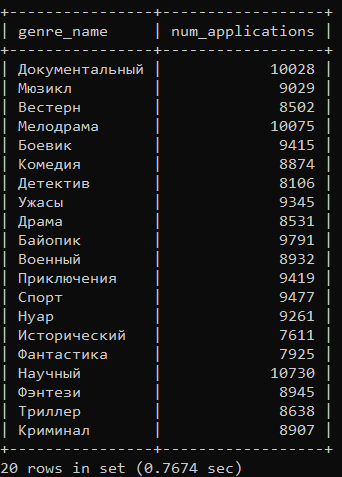
\includegraphics[width=0.5\linewidth]{31.png}
	\caption{Результат выполнения запроса № 3.1}
	\label{fig:31}
\end{figure}

\begin{figure}[H]
	\centering
	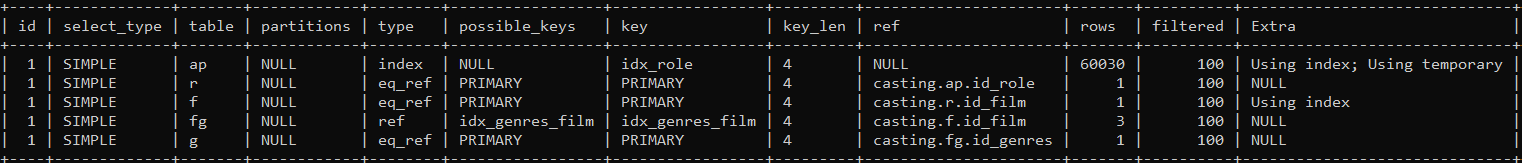
\includegraphics[width=1.0\linewidth]{e31.png}
	\caption{Результат применения команды explain к данному запросу}
	\label{fig:e31}
\end{figure}

\begin{figure}[H]
	\centering
	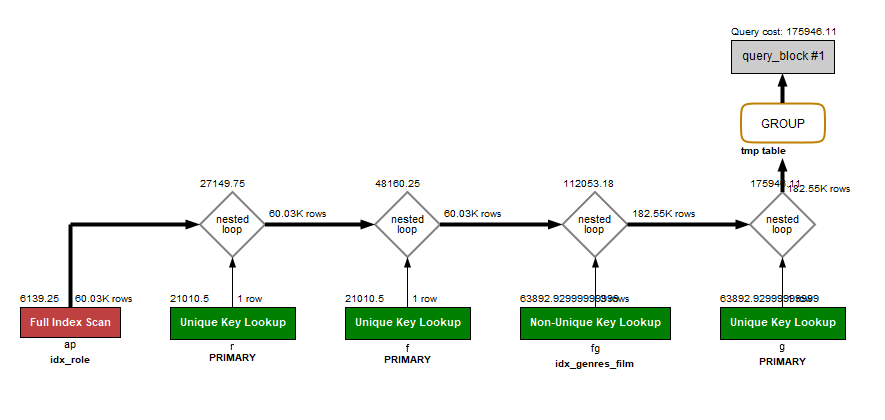
\includegraphics[width=1.0\linewidth]{ex31.png}
	\caption{Графический план выполнения запроса № 3.1.}
	\label{fig:ex31}
\end{figure}

\subsection{Запрос № 3.2}

\par \textbf{Текст запроса на русском}: Для каждого жанра подсчитать число актеров, которые подавали заявки на фильмы. 
\par Текст SQL запроса представлен в листинге 4.

\begin{lstlisting}[caption=SQL запрос № 3.2, language=SQL]
SELECT g.name AS genre_name, COUNT(DISTINCT a.id_actor) AS num_actors
FROM genres g
LEFT JOIN film_genres fg ON g.id_genres = fg.id_genres
LEFT JOIN film f ON fg.id_film = f.id_film
LEFT JOIN role r ON f.id_film = r.id_film
LEFT JOIN application ap ON r.id_role = ap.id_role
LEFT JOIN actor a ON ap.id_actor = a.id_actor
GROUP BY g.id_genres, g.name;
\end{lstlisting}

\par В качестве результата выполнения запроса была получена таблица на 20 строк. Запрос выполнился за 0.7518 секунд. Таблица с результатами представлена на \autoref{fig:32}.

\newpage
\begin{figure}[H]
	\centering
	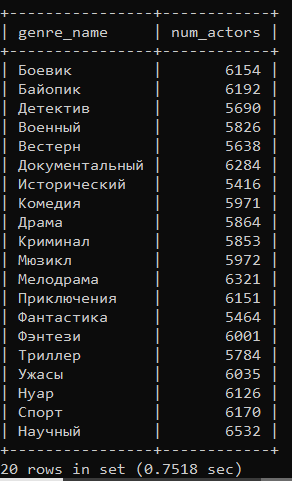
\includegraphics[width=0.3\linewidth]{32.png}
	\caption{Результат выполнения запроса № 3.2}
	\label{fig:32}
\end{figure}

\begin{figure}[H]
	\centering
	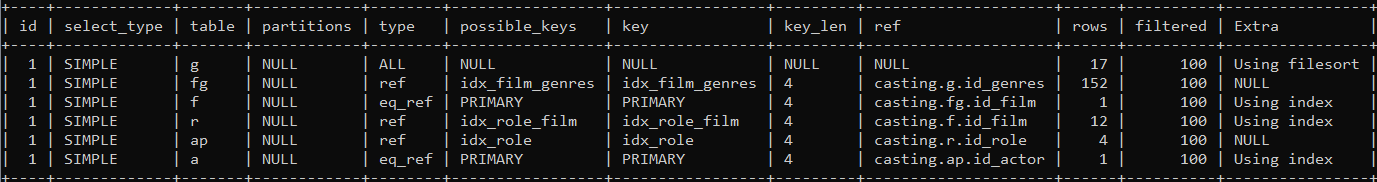
\includegraphics[width=1.0\linewidth]{e32.png}
	\caption{Результат применения команды explain к данному запросу}
	\label{fig:e32}
\end{figure}

\begin{figure}[H]
	\centering
	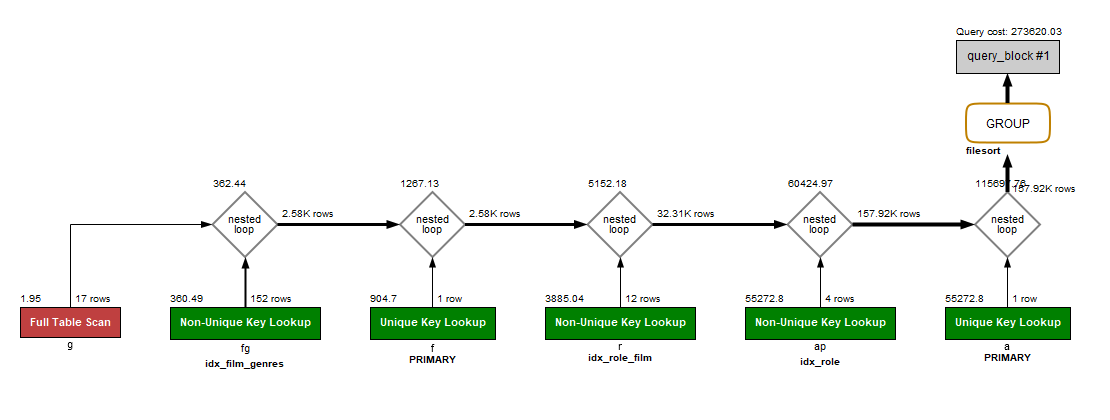
\includegraphics[width=1.0\linewidth]{ex32.png}
	\caption{Графический план выполнения запроса № 3.2.}
	\label{fig:ex32}
\end{figure}

\begin{figure}[H]
	\centering
	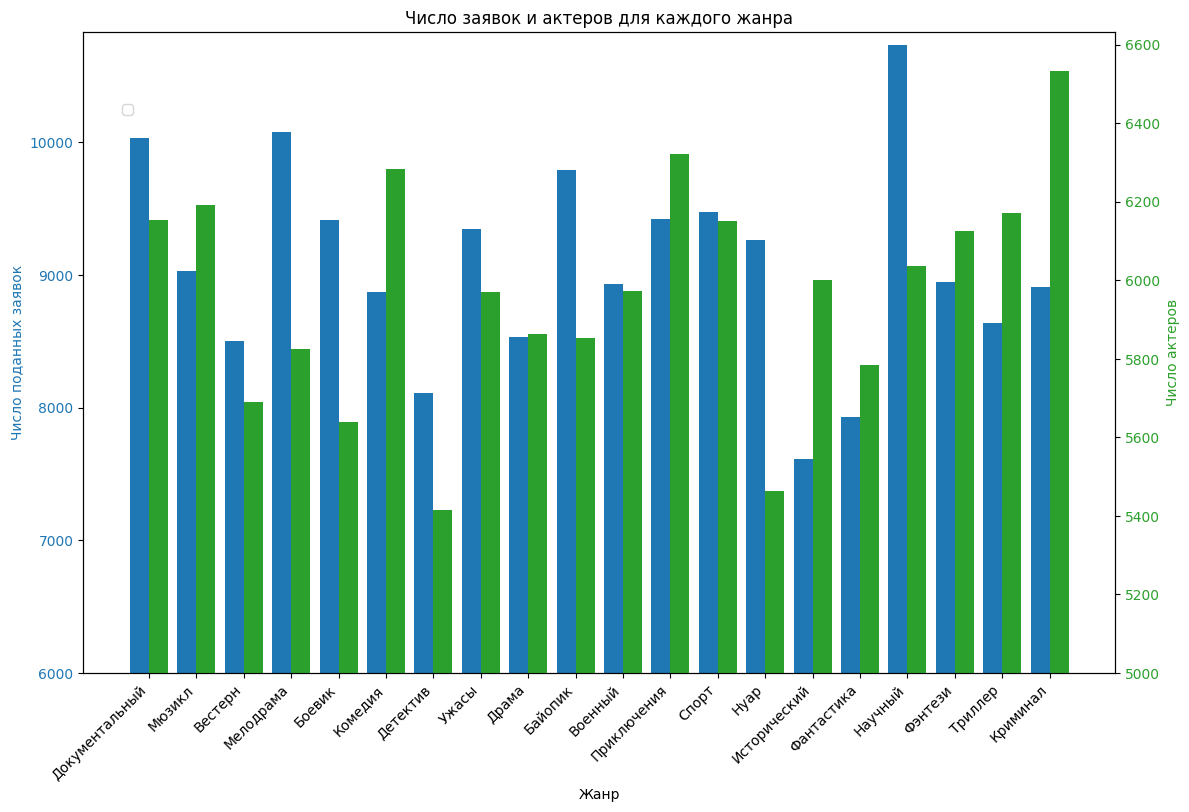
\includegraphics[width=1.0\linewidth]{d3.png}
	\caption{Число актеров и заявок для каждого жанра}
	\label{fig:d3}
\end{figure}


\subsection{Запрос № 4}

\par \textbf{Текст запроса на русском}: Подсчитать число режиссеров с одиннаковым числом заявок. 
\par Текст SQL запроса представлен в листинге 5.

\begin{lstlisting}[caption=SQL запрос № 4, language=SQL]
	SELECT COUNT(id_director) AS num_directors, num_apps
	FROM (
	SELECT id_director, COUNT(*) AS num_apps
	FROM application
	GROUP BY id_director
	) AS director_apps_count
	GROUP BY num_apps
	ORDER BY num_apps ASC;
\end{lstlisting}

\par В качестве результата выполнения запроса была получена таблица на 16 строк. Запрос выполнился за 0.0396 секунд. Таблица с результатами представлена на \autoref{fig:4}.

\begin{figure}[H]
	\centering
	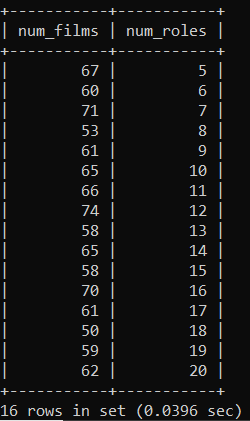
\includegraphics[width=0.25\linewidth]{4.png}
	\caption{Результат выполнения запроса № 4}
	\label{fig:4}
\end{figure}

\begin{figure}[H]
	\centering
	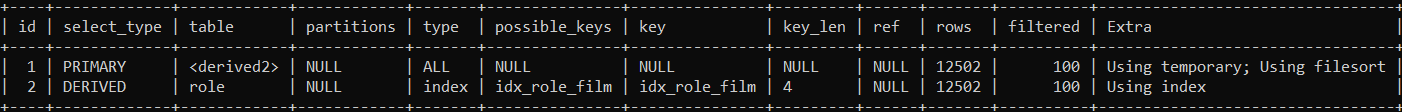
\includegraphics[width=1.0\linewidth]{e4.png}
	\caption{Результат применения команды explain к данному запросу}
	\label{fig:e4}
\end{figure}

\begin{figure}[H]
	\centering
	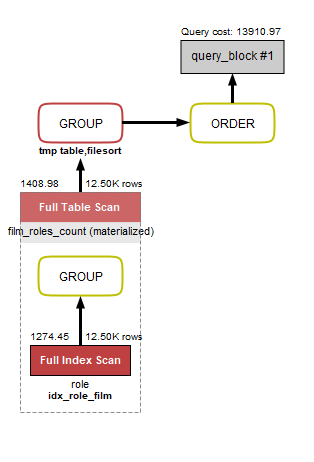
\includegraphics[width=0.4\linewidth]{ex4.png}
	\caption{Графический план выполнения запроса № 4.}
	\label{fig:ex4}
\end{figure}

\begin{figure}[H]
	\centering
	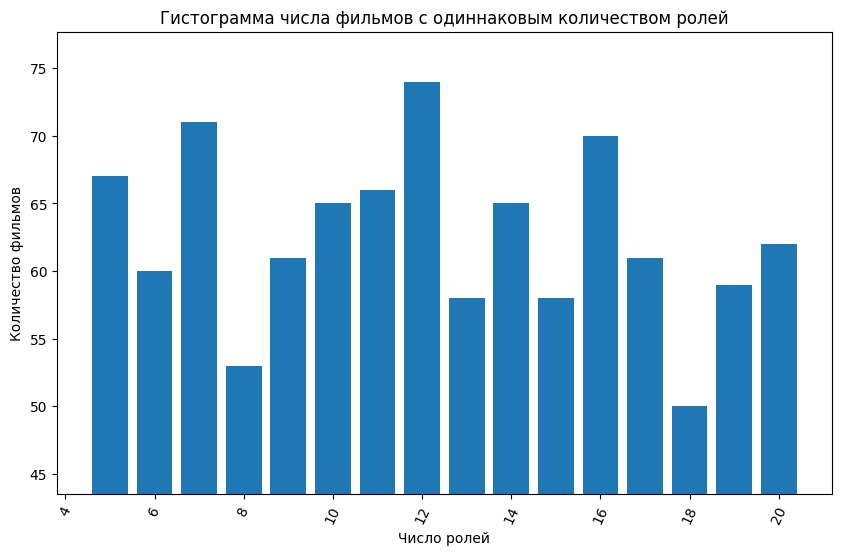
\includegraphics[width=0.7\linewidth]{g4.png}
	\caption{Гистограмма числа фильмов с одиннаковым количеством ролей}
	\label{fig:g4}
\end{figure}


\subsection{Запрос № 5}

\par \textbf{Текст запроса на русском}: Найти кастинг-директоров, который рассматривает заявок больше, чем кастинг-директор А.  
\par Текст SQL запроса представлен в листинге 6.

\begin{lstlisting}[caption=SQL запрос № 5, language=SQL]
   SELECT cd.id_casting_director, cd.surname, cd.name, COUNT(a.id_application) AS num_applications
   FROM casting_director cd
   JOIN application a ON cd.id_casting_director = a.id_casting_director
   GROUP BY cd.id_casting_director, cd.surname, cd.name
   HAVING num_applications > (
   SELECT COUNT(id_application)
   FROM application
   WHERE id_casting_director = 1
   )
   ORDER BY num_applications ASC;
\end{lstlisting}


\par В качестве результата выполнения запроса была получена таблица на 89 строк. Запрос выполнился за 0.0936 секунд. Таблица с результатами представлена на \autoref{fig:51} и \autoref{fig:52}.

\newpage
\begin{figure}[H]
	\centering
	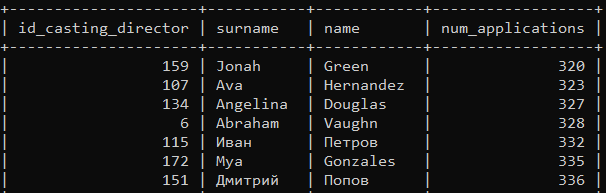
\includegraphics[width=0.7\linewidth]{51.png}
	\caption{Результат выполнения запроса № 5}
	\label{fig:51}
\end{figure}

\begin{figure}[H]
	\centering
	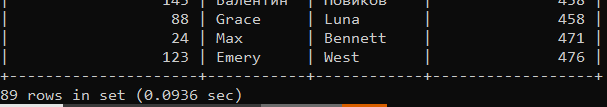
\includegraphics[width=0.7\linewidth]{52.png}
	\caption{Результат выполнения запроса № 5}
	\label{fig:52}
\end{figure}

\begin{figure}[H]
	\centering
	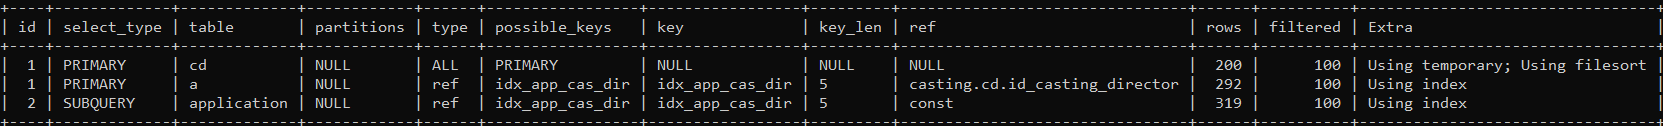
\includegraphics[width=1.0\linewidth]{e5.png}
	\caption{Результат применения команды explain к данному запросу}
	\label{fig:e5}
\end{figure}

\begin{figure}[H]
	\centering
	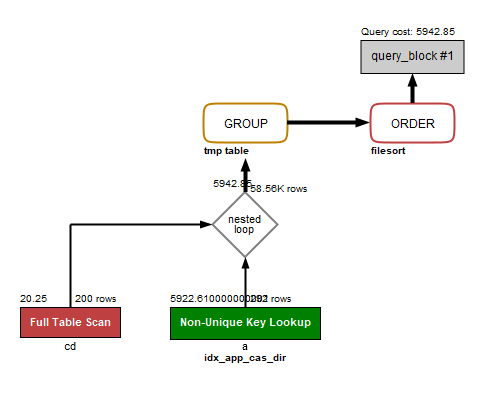
\includegraphics[width=0.65\linewidth]{ex5.png}
	\caption{Графический план выполнения запроса № 5.}
	\label{fig:ex5}
\end{figure}
\newpage
\subsection{Запрос № 6.1}

\par \textbf{Текст запроса на русском}: Найти режиссеров, которые режиссировали максимальное число фильмов. 
\par Текст SQL запроса представлен в листинге 7.

\begin{lstlisting}[caption=SQL запрос № 6.1, language=SQL]
    SELECT d.id_director, d.name, d.surname, COUNT(f.id_film) AS total_films
    FROM director d
    JOIN film f ON d.id_director = f.id_director
    GROUP BY d.id_director, d.name, d.surname
    HAVING total_films = (
        SELECT COUNT(*)
        FROM film
        GROUP BY id_director
        ORDER BY COUNT(*) DESC
        LIMIT 1
    );
\end{lstlisting}


\par В качестве результата выполнения запроса была получена таблица на 108 строк. Запрос выполнился за 0.0062 секунд. Таблица с результатами представлена на \autoref{fig:61} и \autoref{fig:62}.

\begin{figure}[H]
	\centering
	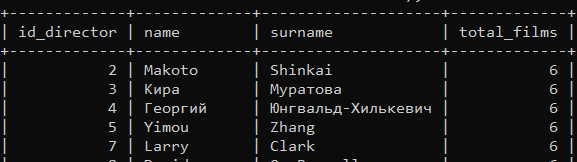
\includegraphics[width=0.7\linewidth]{61.png}
	\caption{Результат выполнения запроса № 6.1}
	\label{fig:61}
\end{figure}

\begin{figure}[H]
	\centering
	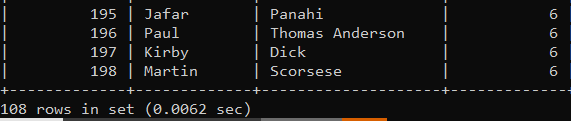
\includegraphics[width=0.7\linewidth]{62.png}
	\caption{Результат выполнения запроса № 6.1}
	\label{fig:62}
\end{figure}

\begin{figure}[H]
	\centering
	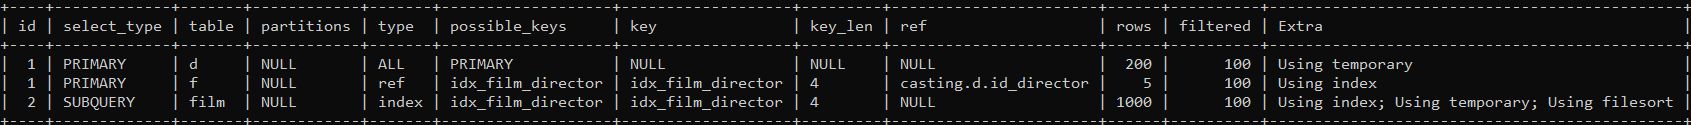
\includegraphics[width=1.0\linewidth]{e61.png}
	\caption{Результат применения команды explain к данному запросу}
	\label{fig:e61}
\end{figure}

\begin{figure}[H]
	\centering
	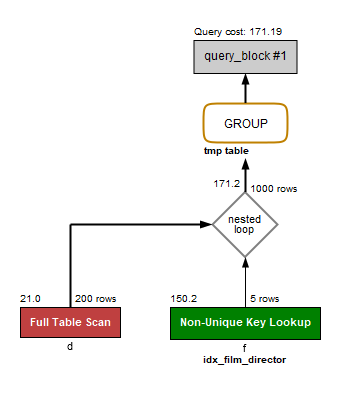
\includegraphics[width=0.6\linewidth]{ex61.png}
	\caption{Графический план выполнения запроса № 6.1.}
	\label{fig:ex61}
\end{figure}

\subsection{Запрос № 6.2}

\par \textbf{Текст запроса на русском}: Найти режиссеров, которые режиссировали минимальное число фильмов. 
\par Текст SQL запроса представлен в листинге 8.

\begin{lstlisting}[caption=SQL запрос № 6.2, language=SQL]
    SELECT d.id_director, d.name, d.surname, COUNT(f.id_film) AS total_films
    FROM director d
    JOIN film f ON d.id_director = f.id_director
    GROUP BY d.id_director, d.name, d.surname
    HAVING total_films = (
        SELECT COUNT(*)
        FROM film
        GROUP BY id_director
        ORDER BY COUNT(*) ASC
        LIMIT 1
    );
\end{lstlisting}


\par В качестве результата выполнения запроса была получена таблица на 5 строк. Запрос выполнился за 0.0045 секунд. Таблица с результатами представлена на \autoref{fig:63}.

\begin{figure}[H]
	\centering
	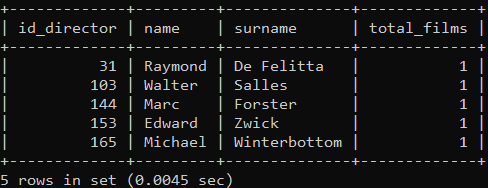
\includegraphics[width=0.7\linewidth]{63.png}
	\caption{Результат выполнения запроса № 6.2}
	\label{fig:63}
\end{figure}


\begin{figure}[H]
	\centering
	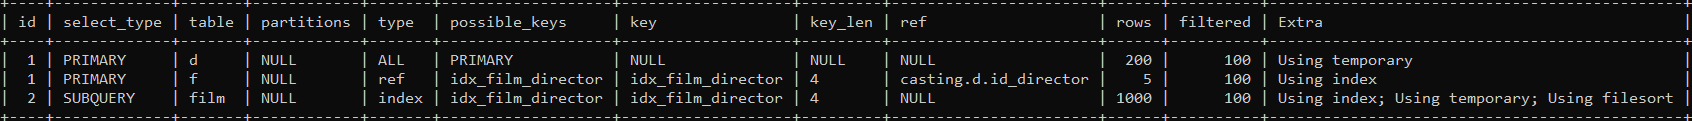
\includegraphics[width=1.0\linewidth]{e62.png}
	\caption{Результат применения команды explain к данному запросу}
	\label{fig:e62}
\end{figure}

\begin{figure}[H]
	\centering
	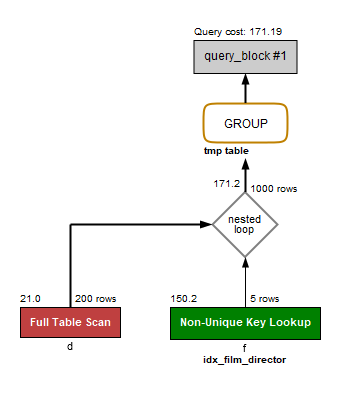
\includegraphics[width=0.5\linewidth]{ex62.png}
	\caption{Графический план выполнения запроса № 6.2.}
	\label{fig:ex62}
\end{figure}

\subsection{Запрос № 7}

\par \textbf{Текст запроса на русском}: Найти актеров, которые участвовали, но не прошли парные пробы. 
\par Текст SQL запроса представлен в листинге 9.

\begin{lstlisting}[caption=SQL запрос № 7, language=SQL]
	SELECT a.surname, a.name, COUNT(da.id_application) AS num_double_auditions,  
	                                                      da.getting_a_role
	FROM actor a
	JOIN application ap ON a.id_actor = ap.id_actor
	JOIN doubles_audition da ON ap.id_application = da.id_application
	WHERE da.getting_a_role = 'Роль не получена'
	GROUP BY a.id_actor, a.surname, a.name
	HAVING num_double_auditions < (
	   SELECT COUNT(id_doubles_audition)
	   FROM doubles_audition
  	   WHERE getting_a_role = 'Роль не получена'
	);
\end{lstlisting}

\par В качестве результата выполнения запроса была получена таблица на 6863 строк. Запрос выполнился за 0.1013 секунд. Таблица с результатами представлена на \autoref{fig:71} и \autoref{fig:72}.

\begin{figure}[H]
	\centering
	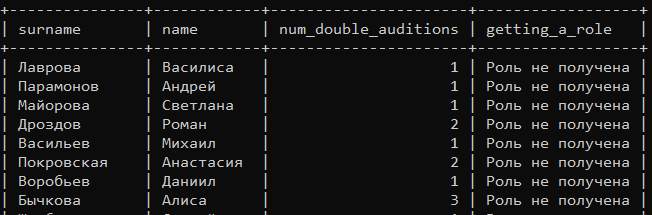
\includegraphics[width=0.7\linewidth]{71.png}
	\caption{Результат выполнения запроса № 7}
	\label{fig:71}
\end{figure}

\begin{figure}[H]
	\centering
	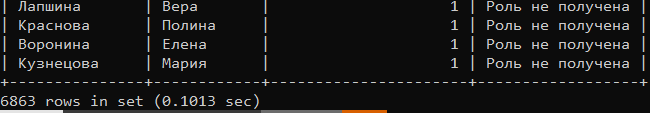
\includegraphics[width=0.7\linewidth]{72.png}
	\caption{Результат выполнения запроса № 7}
	\label{fig:72}
\end{figure}

\begin{figure}[H]
	\centering
	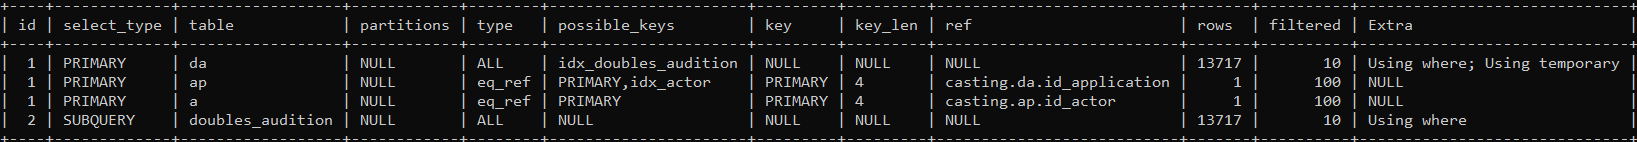
\includegraphics[width=1.0\linewidth]{e7.png}
	\caption{Результат применения команды explain к данному запросу}
	\label{fig:e7}
\end{figure}

\begin{figure}[H]
	\centering
	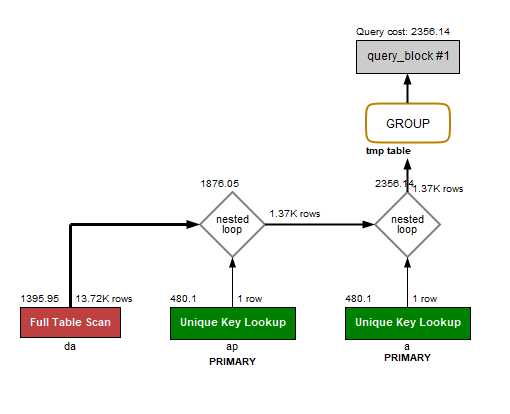
\includegraphics[width=0.55\linewidth]{ex7.png}
	\caption{Графический план выполнения запроса № 7.}
	\label{fig:ex7}
\end{figure}

\subsection{Запрос № 8}

\par \textbf{Текст запроса на русском}: Для каждого типа роли и каждого режиссера подсчитать число заявок.
\par Текст SQL запроса представлен в листинге 10.

\begin{lstlisting}[caption=SQL запрос № 8, language=SQL]

SELECT 
   role_type.name AS role_type, 
   director.surname AS Dir_surname, 
   director.name AS Dir_name,
   (  
      SELECT COUNT(ap.id_application)
      FROM application ap
      JOIN role r ON ap.id_role = r.id_role
      WHERE director.id_director = ap.id_director AND id_role_type = r.id_role_type
   ) AS num_applications
FROM
   role_type
CROSS JOIN
   director
ORDER BY
   role_type;    	
	
\end{lstlisting}

\par В качестве результата выполнения запроса была получена таблица на 600 строк. Запрос выполнился за 0.5176 секунд. Таблица с результатами представлена на \autoref{fig:81} и \autoref{fig:82}.


\begin{figure}[H]
	\centering
	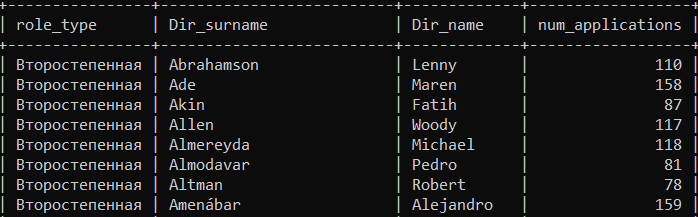
\includegraphics[width=0.6\linewidth]{81.png}
	\caption{Результат выполнения запроса № 8}
	\label{fig:81}
\end{figure}

\begin{figure}[H]
	\centering
	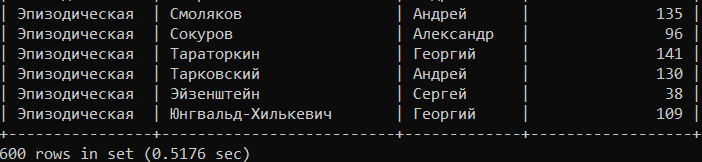
\includegraphics[width=0.6\linewidth]{82.png}
	\caption{Результат выполнения запроса № 8}
	\label{fig:82}
\end{figure}


\begin{figure}[H]
	\centering
	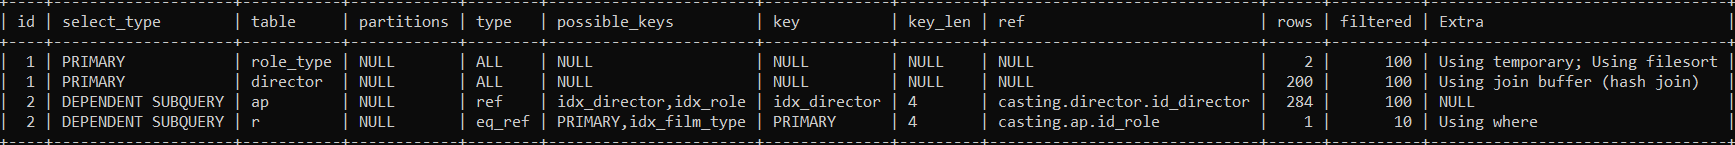
\includegraphics[width=1.0\linewidth]{e8.png}
	\caption{Результат применения команды explain к данному запросу}
	\label{fig:e8}
\end{figure}

\begin{figure}[H]
	\centering
	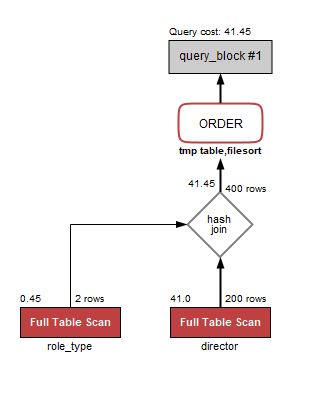
\includegraphics[width=0.5\linewidth]{ex8.png}
	\caption{Графический план выполнения запроса № 8.}
	\label{fig:ex8}
\end{figure}

\includepdf[pages=-,fitpaper]{gist.pdf} % Вставка документа формата A3  


\newpage
\section*{Заключение}
\addcontentsline{toc}{section}{Заключение}

\par В первой части была выбрана и изучена предметная область, связанная с процессом прохождения кастинга актером на роль в фильме. Были выделены 7 сущностей и 3 роли. У каждой сущности и каждой роли присутствуют свои атрибуты. Для лучшего описания связей между сущностями была создана ER-диаграмма.

\par Во второй части была создана диаграмма объектов, которая показывает связи будующих таблиц. Также была создана схема данных на русском и английском языках. Данная схема показывает полное соотношение связей между таблицами в базе данных. Для описания каждого объекта в базе данных были созданы таблицы с тимами данных и полями атрибутов. По данным таблицам был составлен код SQL, по которому строятся объекты в базу данных. База данных имеет 12 таблиц, связанных между собой.

\par В третьей части были собраны данные для заполнения базы данных. С помощью языка Python 3.11 и запросов SQL были заполнены имеющиеся таблицы при условии равномерного распределения данных. Общее количество записей в базе данных составляет 203 094 единиц. Также были сделаны 10 запросов в базу данных. Их суть состояла в том, чтобы посчитать определенное количество записей, либо же найти определенные значения полей. 

\par В ходе выполнения курсовой работы была спроектирована и реализована база данных для хранения заявок актеров. 

\par На работу было потрачено около 4-х месяцев. Код заполнения таблиц составляет 597 строк, код запросов 326 строк. 

\par Работа была выполнена в системе управления базами данных MySQL Server 8.0, а также были использованы возможности языка Python 3.11.

\par Полученные опыт и знания будут использоваться в дальнейших работах и проектах. 
\newpage


\section*{Список литературы}
\addcontentsline{toc}{section}{Список литературы} % Добавляем раздел в содержание

[1] Мана Такахаси, Сёко Адзума. Базы данных. - Москва: ДМК Пресс, 2015. - 240 с.

[2] Силверман, Бен. MySQL. Библия пользователя. - М.: ДМК Пресс, 2019. - 928 с.

[3] Бейли, Ларри Ульман. Изучаем MySQL. - 3-е издание. - СПб.: Питер, 2019. - 736 с.

\newpage

\section*{Приложение А. Текст создания БД}	
\addcontentsline{toc}{section}{Приложение А. Текст создания БД} 
\label{sec:appendixA}

\begin{lstlisting}[language=SQL]
CREATE DATABASE casting;
USE casting;

CREATE TABLE IF NOT EXISTS actor (
id_actor INT UNSIGNED NOT NULL AUTO_INCREMENT,
surname varchar(30) COLLATE utf8mb4_unicode_ci DEFAULT NULL,
name varchar(20) COLLATE utf8mb4_unicode_ci DEFAULT NULL,
patronymic varchar(20) COLLATE utf8mb4_unicode_ci DEFAULT NULL,
date_of_birth DATE DEFAULT NULL,
passport_number VARCHAR(10) DEFAULT NULL,
education TEXT COLLATE utf8mb4_unicode_ci DEFAULT NULL,
work_experience TEXT COLLATE utf8mb4_unicode_ci DEFAULT NULL,
PRIMARY KEY (id_actor)
) ENGINE=InnoDB DEFAULT CHARSET=utf8mb4 COLLATE=utf8mb4_unicode_ci 
  AUTO_INCREMENT=1;


CREATE TABLE IF NOT EXISTS application (
id_application INT UNSIGNED NOT NULL AUTO_INCREMENT,
filmography TEXT COLLATE utf8mb4_unicode_ci DEFAULT NULL,
photos VARCHAR(200) DEFAULT NULL,
id_actor INT UNSIGNED NOT NULL, 
id_role INT UNSIGNED NOT NULL,
id_сasting_director INT UNSIGNED NOT NULL,
id_director INT UNSIGNED NOT NULL,
PRIMARY KEY (id_application),
FOREIGN KEY (id_actor) REFERENCES actor(id_actor), 
FOREIGN KEY (id_role) REFERENCES role(id_role),
FOREIGN KEY(id_сasting_director) REFERENCES casting_director(id_casting_director),
FOREIGN KEY(id_director) REFERENCES director(id_director)
) ENGINE=InnoDB DEFAULT CHARSET=utf8mb4 COLLATE=utf8mb4_unicode_ci 
  AUTO_INCREMENT=1;


CREATE TABLE IF NOT EXISTS director(
id_director INT UNSIGNED NOT NULL AUTO_INCREMENT,
surname varchar(30) COLLATE utf8mb4_unicode_ci DEFAULT NULL,
name varchar(20) COLLATE utf8mb4_unicode_ci DEFAULT NULL,
patronymic varchar(20) COLLATE utf8mb4_unicode_ci DEFAULT NULL,
date_of_birth DATE DEFAULT NULL,
passport_number VARCHAR(10) DEFAULT NULL,
filmography TEXT COLLATE utf8mb4_unicode_ci DEFAULT NULL,
PRIMARY KEY (id_director)
) ENGINE=InnoDB DEFAULT CHARSET=utf8mb4 COLLATE=utf8mb4_unicode_ci 
  AUTO_INCREMENT=1;


CREATE TABLE IF NOT EXISTS casting_director (
id_casting_director INT UNSIGNED NOT NULL AUTO_INCREMENT,
surname varchar(30) COLLATE utf8mb4_unicode_ci DEFAULT NULL,
name varchar(20) COLLATE utf8mb4_unicode_ci DEFAULT NULL,
patronymic varchar(20) COLLATE utf8mb4_unicode_ci DEFAULT NULL,
date_of_birth DATE DEFAULT NULL,
passport_number VARCHAR(10) DEFAULT NULL,
filmography TEXT COLLATE utf8mb4_unicode_ci DEFAULT NULL,
PRIMARY KEY (id_casting_director)
) ENGINE=InnoDB DEFAULT CHARSET=utf8mb4 COLLATE=utf8mb4_unicode_ci 
  AUTO_INCREMENT=1;


CREATE TABLE IF NOT EXISTS role (
id_role INT UNSIGNED NOT NULL AUTO_INCREMENT,
name varchar(30) COLLATE utf8mb4_unicode_ci DEFAULT NULL,
discription TEXT COLLATE utf8mb4_unicode_ci DEFAULT NULL,
id_role_type INT UNSIGNED  NOT NULL, 
id_film INT UNSIGNED  NOT NULL, 
FOREIGN KEY(id_role_type) REFERENCES role_type(id_role_type),
FOREIGN KEY(id_film) REFERENCES film(id_film), 
PRIMARY KEY (id_role)
) ENGINE=InnoDB DEFAULT CHARSET=utf8mb4 COLLATE=utf8mb4_unicode_ci 
  AUTO_INCREMENT=1;


CREATE TABLE IF NOT EXISTS role_type (
id_role_type INT UNSIGNED NOT NULL AUTO_INCREMENT,
name varchar(15) COLLATE utf8mb4_unicode_ci DEFAULT NULL,
PRIMARY KEY (id_role_type)
) ENGINE=InnoDB DEFAULT CHARSET=utf8mb4 COLLATE=utf8mb4_unicode_ci   
  AUTO_INCREMENT=1;	


CREATE TABLE IF NOT EXISTS film (
id_film INT UNSIGNED NOT NULL AUTO_INCREMENT,
name varchar(30) COLLATE utf8mb4_unicode_ci DEFAULT NULL,
id_director INT UNSIGNED  NOT NULL, 
id_casting_director INT UNSIGNED NOT NULL,
FOREIGN KEY(id_director) REFERENCES director(id_director),
FOREIGN KEY(id_casting_director) REFERENCES casting_director(id_casting_director), 
PRIMARY KEY (id_film)
) ENGINE=InnoDB DEFAULT CHARSET=utf8mb4 COLLATE=utf8mb4_unicode_ci 
  AUTO_INCREMENT=1;


CREATE TABLE IF NOT EXISTS film_genres (
id_film_genres INT UNSIGNED NOT NULL AUTO_INCREMENT,
PRIMARY KEY (id_film_genres),
id_film INT UNSIGNED NOT NULL,
id_genres INT UNSIGNED NOT NULL,
FOREIGN KEY(id_film) REFERENCES film(id_film), 
FOREIGN KEY(id_genres) REFERENCES genres(id_genres) 
) ENGINE=InnoDB DEFAULT CHARSET=utf8mb4 COLLATE=utf8mb4_unicode_ci 
  AUTO_INCREMENT=1;


CREATE TABLE IF NOT EXISTS genres (
id_genres INT UNSIGNED NOT NULL AUTO_INCREMENT,
name VARCHAR(20) COLLATE utf8mb4_unicode_ci DEFAULT NULL,
PRIMARY KEY (id_genres)
) ENGINE=InnoDB DEFAULT CHARSET=utf8mb4 COLLATE=utf8mb4_unicode_ci 
  AUTO_INCREMENT=1;


CREATE TABLE IF NOT EXISTS first_stage (
id_first_stage INT UNSIGNED NOT NULL AUTO_INCREMENT,
directors_assessment TINYINT UNSIGNED DEFAULT NULL, 
casting_directors_assesment TINYINT UNSIGNED DEFAULT NULL,
id_application INT UNSIGNED NOT NULL,  
PRIMARY KEY (id_first_stage),
FOREIGN KEY(id_application) REFERENCES application(id_application) 
) ENGINE=InnoDB DEFAULT CHARSET=utf8mb4 COLLATE=utf8mb4_unicode_ci 
  AUTO_INCREMENT=1;


CREATE TABLE IF NOT EXISTS audition (
id_audition INT UNSIGNED NOT NULL AUTO_INCREMENT,
directors_assessment TINYINT UNSIGNED DEFAULT NULL, 
casting_directors_assesment TINYINT UNSIGNED DEFAULT NULL,
id_application INT UNSIGNED NOT NULL,  
PRIMARY KEY (id_audition),
FOREIGN KEY(id_application) REFERENCES application(id_application) 
) ENGINE=InnoDB DEFAULT CHARSET=utf8mb4 COLLATE=utf8mb4_unicode_ci 
  AUTO_INCREMENT=1;


CREATE TABLE IF NOT EXISTS doubles_audition (
id_doubles_audition INT UNSIGNED NOT NULL AUTO_INCREMENT,
directors_assessment TINYINT UNSIGNED DEFAULT NULL, 
casting_directors_assesment TINYINT UNSIGNED DEFAULT NULL,
i  
id_application INT UNSIGNED NOT NULL,
PRIMARY KEY (id_doubles_audition),
FOREIGN KEY(id_application) REFERENCES application(id_application)
) ENGINE=InnoDB DEFAULT CHARSET=utf8mb4 COLLATE=utf8mb4_unicode_ci 
  AUTO_INCREMENT=1;	
	
\end{lstlisting}	


\section*{Приложение Б. Текст программы для заполнения таблиц в БД}
\addcontentsline{toc}{section}{Приложение Б. Текст программы для заполнения таблиц в БД}
\label{sec:appendixB}

\subsection*{Приложение Б.1. Заполнение таблицы "actor"}	

\begin{lstlisting}	

import pymysql
import random
from datetime import datetime
def random_date():
year = random.randint(1980, 2006)
month = random.randint(1, 12)
day = random.randint(1, 28)
return datetime(year, month, day).date()

def generate_passport():
first_part = ''.join(random.choices('0123456789', k=4))
second_part = ''.join(random.choices('0123456789', k=6))
passport_number = f"{first_part} {second_part}"
return passport_number

def generate_education():
with open("uni.txt", "r", encoding="utf-8") as uni_file,
     open("education.txt", "r", encoding="utf-8") as education_file:
edu = education_file.readlines()
uni = uni_file.readlines()
random_edu = random.choice(edu)

if "Высшее образование" in random_edu:
rand_uni = random.choice(uni)
else:
rand_uni = ""

result_str = random_edu.strip() + " " + rand_uni.strip()
return result_str

def generate_work():
with open("work_experience.txt", "r", encoding="utf-8") as work_file:
work = work_file.readlines()
random_work = random.choice(work)
return random_work.strip()

host = 'localhost'
user = 'root'
password = 'A1l2e3k4s5e6y7'
db_name = 'casting'

try:
connection = pymysql.connect(
host=host,
port=3306,
user=user,
password=password,
database=db_name,
cursorclass=pymysql.cursors.DictCursor
)
print("successfully connected...")
print("#" * 20)

names_file = open("fullnames.txt", "r", encoding="utf-8")
names = names_file.readlines()
names_file.close()
random.shuffle(names)
rand_names = []
for line in names:
parts = line.split()
rand_names.append(parts)

for i in range(10000):
index = random.randint(0, len(names) - 1)

date = random_date()
passport = generate_passport()
education = generate_education()
work = generate_work()

try:
with connection.cursor() as cursor:
insert_query = ("INSERT INTO actor (surname, name, patronymic, date_of_birth, "
"passport_number, education, work_experience) "
" VALUES (%s, %s, %s, %s, %s, %s, %s)")
cursor.execute(insert_query, (rand_names[index][0], rand_names[index][1], rand_names[index][2],
date, passport, education, work))
connection.commit()

finally: 
   pass

connection.close()
except Exception as ex:
print("Connection refused")
print(ex)

\end{lstlisting}

\subsection*{Приложение Б.2. Заполнение таблиц 'director' и 'casting\_director'}

\begin{lstlisting}

import pymysql
import random
from datetime import datetime

def generate_award():
with open("awards.txt", "r", encoding="utf-8") as awards_file:
awards = awards_file.readlines()
random_award = random.choice(awards)
return random_award.strip()

host = 'localhost'
user = 'root'
password = 'A1l2e3k4s5e6y7'
db_name = 'casting'

try:
connection = pymysql.connect(
host=host,
port=3306,
user=user,
password=password,
database=db_name,
cursorclass=pymysql.cursors.DictCursor
)
print("successfully connected...")
print("#" * 20)

dir_file = open("casting_dir.txt", "r", encoding="utf-8")
directors = dir_file.readlines()
dir_file.close()
random.shuffle(directors)
dr = []
for line in directors:
parts = line.strip().split(maxsplit=1)
dr.append(parts)

for i in range(200):
date = random_date()
passport = generate_passport()

try:
with connection.cursor() as cursor:
insert_query = ("INSERT INTO casting_director (name, surname, date_of_birth, passport_number) "
" VALUES (%s, %s, %s, %s)")
cursor.execute(insert_query, (dr[i][0], dr[i][1], date, passport))
connection.commit()

finally: pass
connection.close()

except Exception as ex:
print("Connection refused")
print(ex)	
	
\end{lstlisting}

	
	
\subsection*{Приложение Б.3. Заполнение таблицы 'film'}

\begin{lstlisting}	
import pymysql
import random

host = 'localhost'
user = 'root'
password = 'A1l2e3k4s5e6y7'
db_name = 'casting'

try:
connection = pymysql.connect(
host=host,
port=3306,
user=user,
password=password,
database=db_name,
cursorclass=pymysql.cursors.DictCursor
)
print("successfully connected...")
print("#" * 20)

film_file = open("films.txt", "r", encoding="utf-8")
films = [line.strip() for line in film_file.readlines()]
film_file.close()
random.shuffle(films)

count_dir = [0] * 201
count_cas = [0] * 201

for i in range(1000):

dir = random.randint(1, 200)
while (count_dir[dir] > 5):
dir = random.randint(1, 200)
count_dir[dir] += 1

cas = random.randint(1, 200)
while (count_cas[cas] > 5):
cas = random.randint(1, 200)
count_cas[cas] += 1

try:
with connection.cursor() as cursor:
insert_query = ("INSERT INTO film (name, id_director, id_casting_director) "
" VALUES (%s, %s, %s)")
cursor.execute(insert_query, (films[i], dir, cas))
connection.commit()

finally: pass
connection.close()

except Exception as ex:
print("Connection refused")
print(ex)

\end{lstlisting}
	

\subsection*{Приложение Б.4. Заполнение таблицы 'genres'} 

\begin{lstlisting}	
	
import pymysql

# Подключение к базе данных
def connect_to_db():
host = 'localhost'
user = 'root'
password = 'A1l2e3k4s5e6y7'
db_name = 'casting'

connection = pymysql.connect(
host=host,
port=3306,
user=user,
password=password,
database=db_name,
cursorclass=pymysql.cursors.DictCursor
)
return connection

def add_genre(connection, name):
try:
  with connection.cursor() as cursor:
  sql = "INSERT INTO genres (name) VALUES (%s)"
  cursor.execute(sql, (name,))
# Фиксация изменений в базе данных
  connection.commit()
  print(f"Жанр '{name}' успешно добавлен в базу данных!")
  except Exception as e:
  print(f"Ошибка при добавлении жанра: {e}")

# Основная функция
def main():
# Список жанров для добавления
genres = [
"Боевик",
"Байопик",
"Детектив",
"Военный",
"Вестерн",
"Документальный",
"Исторический",
"Комедия",
"Драма",
"Криминал",
"Мюзикл",
"Мелодрама",
"Приключения",
"Фантастика",
"Фэнтези",
"Триллер",
"Ужасы",
"Нуар",
"Спорт",
"Научный"
]

connection = connect_to_db()
for genre in genres:
add_genre(connection, genre)

connection.close()

\end{lstlisting}


\subsection*{Приложение Б.5. Заполнение таблицы 'role'}

\begin{lstlisting}	
	
import pymysql
import random

host = 'localhost'
user = 'root'
password = 'A1l2e3k4s5e6y7'
db_name = 'casting'

try:
connection = pymysql.connect(
host=host,
port=3306,
user=user,
password=password,
database=db_name,
cursorclass=pymysql.cursors.DictCursor
)
print("successfully connected...")
print("#" * 20)

role_file = open("roles.txt", "r", encoding="utf-8")
roles = [line.strip() for line in role_file.readlines()]
role_file.close()

for i in range(1000):

count = random.randint(5, 20)
for j in range(count):
index = random.randint(0, len(roles) - 1)
role = roles.pop(index)
role_type = random.randint(1, 3)

try:
with connection.cursor() as cursor:
insert_query = ("INSERT INTO role (name, id_role_type, id_film) "
" VALUES (%s, %s, %s)")
cursor.execute(insert_query, (role, role_type, i + 1))
connection.commit()

finally:
pass

connection.close()

except Exception as ex:
print("Connection refused")
print(ex)
	
\end{lstlisting}


\subsection*{Приложение Б.5. Заполнение таблицы 'role\_type'}

\begin{lstlisting}[language=SQL]	
	
INSERT INTO role_type (name) VALUES ('Главная');
INSERT INTO role_type (name) VALUES ('Второстепенная');
INSERT INTO role_type (name) VALUES ('Эпизодическая');
	
\end{lstlisting}


\subsection*{Приложение Б.6. Заполнение таблицы 'film\_genres'}

\begin{lstlisting}	

import pymysql
import random

host = 'localhost'
user = 'root'
password = 'A1l2e3k4s5e6y7'
db_name = 'casting'

try:
connection = pymysql.connect(
host=host,
port=3306,
user=user,
password=password,
database=db_name,
cursorclass=pymysql.cursors.DictCursor
)
print("successfully connected...")
print("#" * 20)

for i in range(1000):
count = random.randint(1, 5)
for j in range (count):
id_genre = random.randint(1, 20)
try:
with connection.cursor() as cursor:
insert_query = ("INSERT INTO film_genres (id_film, id_genres) "
" VALUES (%s, %s)")
cursor.execute(insert_query, (i + 1, id_genre))
connection.commit()

finally:
pass

connection.close()

except Exception as ex:
print("Connection refused")
print(ex)	
	
\end{lstlisting}


\subsection*{Приложение Б.7. Заполнение таблицы 'application'}
	
\begin{lstlisting}	
import pymysql
import random

host = 'localhost'
user = 'root'
password = 'A1l2e3k4s5e6y7'
db_name = 'casting'

try:
connection = pymysql.connect(
host=host,
port=3306,
user=user,
password=password,  
database=db_name,
cursorclass=pymysql.cursors.DictCursor
)
print("successfully connected...")
print("#" * 20)

f1_file = open("f1.txt", "r", encoding="utf-8")
f1 = [line.strip() for line in f1_file.readlines()]
f1_file.close()

f2_file = open("f2.txt", "r", encoding="utf-8")
f2 = [line.strip() for line in f2_file.readlines()]
f2_file.close()

photodir = "C:/Documents/Photos/actor/"

for i in range(10000):
count = random.randint(5, 7)
film1 = random.choice(f1)
film2 = random.choice(f2)
filmography = film1 + film2

for j in range(count):
role_id = random.randint(1, 12381)
photo = photodir + str(i + 1)

try:
with connection.cursor() as cursor:

cursor.execute("SELECT id_film FROM role WHERE id_role = %s", (role_id,))
result = cursor.fetchone()

film_id = result['id_film']
cursor.execute("SELECT id_director FROM film WHERE id_film = %s", (film_id,))
dir_result = cursor.fetchone()
cursor.execute("SELECT id_casting_director FROM film WHERE id_film = %s", (film_id,))
cas_result = cursor.fetchone()

id_dir = dir_result['id_director']
id_cas = cas_result['id_casting_director']

insert_query = ("INSERT INTO application (filmography, photos, id_actor, id_role, "
" id_casting_director, id_director)"
" VALUES (%s, %s, %s, %s, %s, %s)")
cursor.execute(insert_query, (filmography, photo, i + 1, role_id, id_cas, id_dir))
connection.commit()

finally: pass
connection.close()

except Exception as ex:
print("Connection refused")
print(ex)

\end{lstlisting}
	
	
\subsection*{Приложение Б.8. Заполнение таблицы 'first\_stage'}

\begin{lstlisting}	
import pymysql
import random

host = 'localhost'
user = 'root'
password = 'A1l2e3k4s5e6y7'
db_name = 'casting'

try:
connection = pymysql.connect(
host=host,
port=3306,
user=user,
password=password,
database=db_name,
cursorclass=pymysql.cursors.DictCursor
)
print("successfully connected...")
print("#" * 20)

numbers = list(range(1, 59994))
str1 = "Этап пройден"
str2 = "Этап не пройден"

for i in range(59993):
score1 = random.randint(18, 100)
score2 = random.randint(18, 100)

if(len(numbers) > 2):
rand_index = random.randint(1, len(numbers) - 1)
num = numbers.pop(rand_index)
else:
num = numbers[0]

if(score1 + score2 > 100):
passed = str1
else:
passed = str2

try:
with connection.cursor() as cursor:

insert_query = ("INSERT INTO first_stage (directors_assessment, casting_directors_assessment, "
"id_application, passing) "
" VALUES (%s, %s, %s, %s)")
cursor.execute(insert_query, (score1, score2, num, passed))
connection.commit()

finally:
pass

connection.close()

except Exception as ex:
print("Connection refused")
print(ex)
	
\end{lstlisting}	


\subsection*{Приложение Б.9. Заполнение таблицы 'audition'}

\begin{lstlisting}
	
import pymysql
import random
host = 'localhost'
user = 'root'
password = 'A1l2e3k4s5e6y7'
db_name = 'casting'
try:
connection = pymysql.connect(
host=host,
port=3306,
user=user,
password=password,
database=db_name,
cursorclass=pymysql.cursors.DictCursor
)
print("successfully connected...")
print("#" * 20)

str1 = "Этап пройден"
str2 = "Этап не пройден"

try:
with connection.cursor() as cursor:

select_query = "SELECT id_application FROM first_stage WHERE passing = 'Этап пройден'"
cursor.execute(select_query)
results = cursor.fetchall()

for result in results:
id_app = result['id_application']

score1 = random.randint(10, 80)
score2 = random.randint(10, 80)

if (score1 + score2 > 100):
passed = str1
else:
passed = str2

insert_query = ("INSERT INTO audition (directors_assessment, casting_directors_assessment, "
"id_application, passing) "
" VALUES (%s, %s, %s, %s)")
cursor.execute(insert_query, (score1, score2, id_app, passed))
connection.commit()
finally:
pass
connection.close()
except Exception as ex:
print("Connection refused")
print(ex)
	
\end{lstlisting}


\subsection*{Приложение Б.10. Заполнение таблицы 'doubles\_audition'}

\begin{lstlisting}
	import pymysql
	import random
	
	host = 'localhost'
	user = 'root'
	password = 'A1l2e3k4s5e6y7'
	db_name = 'casting'
	
	try:
	connection = pymysql.connect(
	host=host,
	port=3306,
	user=user,
	password=password,
	database=db_name,
	cursorclass=pymysql.cursors.DictCursor
	)
	print("successfully connected...")
	print("#" * 20)
	
	str1 = "Роль получена"
	str2 = "Роль не получена"
	
	try:
	with connection.cursor() as cursor:
	
	select_query = ("SELECT id_application, directors_assessment, casting_directors_assessment"
	" FROM first_stage WHERE passing = 'Этап пройден'")
	cursor.execute(select_query)
	results = cursor.fetchall()
	
	second_query = ("SELECT id_application, directors_assessment, casting_directors_assessment"
	" FROM audition WHERE passing = 'Этап пройден'")
	cursor.execute(second_query)
	second_st = cursor.fetchall()
	
	for sec_result in second_st:
	id_app = sec_result['id_application']
	dir_asm = sec_result['directors_assessment']
	cas_asm = sec_result['casting_directors_assessment']
	
	for result in results:
	if result['id_application'] == id_app:
	second_dir_asm = result['directors_assessment']
	second_cas_asm = result['casting_directors_assessment']
	break
	
	score1 = random.randint(20, 100)
	score2 = random.randint(20, 100)
	
	total = dir_asm + cas_asm + second_dir_asm + second_cas_asm + score1 + score2
	
	if (total > 400):
	passed = str1
	else:
	passed = str2
	
	insert_query = ("INSERT INTO doubles_audition (directors_assessment, casting_directors_assessment, "
	"id_application, results, getting_a_role) "
	" VALUES (%s, %s, %s, %s, %s)")
	cursor.execute(insert_query, (score1, score2, id_app, total, passed))
	connection.commit()
	
	finally:
	pass
	connection.close()
	except Exception as ex:
	print("Connection refused")
	print(ex)
	
\end{lstlisting} 

	
	
	
	
\end{document}
